

\section{The No-collapse Feature of Kent's theory}
We first consider the no-collapse feature of Kent's theory. This is a feature that belongs both to the many-worlds interpretation and to the pilot wave interpretation. In all three interpretations, the quantum state deterministically evolves according to the Schr\"{o}dinger equation. The Schr\"{o}dinger equation itself describes how a quantum state evolves over time when there are no outside influences. The precise formula for the Schr\"{o}dinger equation need not concern us here, but all we need to know is that the Schr\"{o}dinger equation determines a so-called \textbf{unitary operator}\index{unitary operator} $U(t',t)$. What this means is that if a system is in a state $\ket{\psi}$ at time $t$, then it will be in the state $\ket{\psi'}=U(t',t)\ket{\psi}$
at time $t'$. A unitary operator $U$ has the property that if $\ket{\psi'}=U\ket{\psi}$ and $\ket{\chi'}=U\ket{\chi}$, then 
\begin{equation}\label{unitarycond}
\ip{\chi'}{\psi'}=\ip{\chi}{\psi}.\protect\footnotemark
\end{equation}
\footnotetext{A unitary operator $U$ must also be linear so that for any two states $\ket*{\psi}$ and $\ket*{\phi}$ and complex numbers $\alpha$ and $\beta$, we have 
$$U(\alpha\ket*{\psi}+\beta\ket*{\phi})=\alpha U\ket*{\psi}+\beta U\ket*{\phi},$$
 and furthermore, a unitary operator must have the property that it is invertible: there is a linear operator $U^{-1}$ such that $U U^{-1}$ and $U^{-1} U$ are the identity operator $I$, i.e. $U^{-1} U\ket{\psi}=UU^{-1}\ket{\psi}=\ket{\psi}$ for any state $\ket{\psi}$.}Under the Copenhagen interpretation, a system will evolve unitarily for the most part, but there will typically be a non-unitary change in the state describing the system whenever there is a measurement.\footnote{Note that to say that the change in a state is non-unitary when a measurement is made is not to say that there is a non-unitary collapse operator that maps the quantum state to an eigenstate of some observable. Such a mapping would not make sense, since the collapse is not deterministic given the initial state. However, one could have a well-defined mapping from a time value $t$ to the quantum state of the system $\ket*{\psi(t)}$ at time $t$. We then say that a system changes unitarily if and only if there is a unitary operator $U(t_1,t_0)$ for any two times $t_0$ and $t_1$ such that whenever the state of the system at time $t_0$ is given by $\ket*{\psi(t_0)}$, then the state of the system at time $t_1$ must be given by $\ket*{\psi(t_1)}=U(t_1, t_0)\ket*{\psi(t_0)}$, and that for an intermediate time $t$, $U(t_1,t_0)=U(t_1, t)U(t, t_0).$ So to say that the change in a state is non-unitary when a measurement is made is to say that the state $\ket*{\psi(t)}$ describing the system does not change unitarily in the process of making a measurement. Now to see why this is the case under the Copenhagen interpretation, we suppose that at time $t_0$ a system is in the state $\ket*{\psi(t_0)}$ and that as long as no measurements are made up until a time $t\geq t_0$, the state evolves to a state $\ket*{\psi^{(U)}(t)}=U(t,t_0)\ket*{\psi(t_0)}$ where $U(t,t_0)$ is a unitary operator determined by Schr\"{o}dinger's equation. Furthermore, we suppose that there is a measurable quantity with which we associate an observable $\hat{\bm{O}}$ so that whenever the state of the system is an eigenstate of $\hat{\bm{O}}$, the value of the measurable quantity for the system will be a determinate value and equal to the corresponding eigenvalue of $\hat{\bm{O}}$. At time $t_0$, we can express $\ket*{\psi(t_0)}$ as a linear combination
  $$\ket*{\psi(t_0)}=\sum_i c_i\ket*{s_i(t_0)}$$
 where the $\ket*{s_i(t_0)}$ are eigenstates of $\hat{\bm{O}}$ with distinct eigenvalues. As long as no measurement is made, this will evolve as 
 $$\ket*{\psi^{(U)}(t)}=\sum_i c_iU(t,t_0)\ket*{s_i(t_0)}.$$  
 We assume that as the state $\ket*{s_i(t_0)}$ evolves to the state $\ket*{s_i(t_1)}$ from time $t_0$ to $t_1$, it remains an eigenstates of $\hat{\bm{O}}$ with approximately the same eigenvalue. This assumption is based on the principle that in practice, performing a measurement is not instantaneous, but rather must take place over a time interval, and so the eigenstate and eigenvalue must be stable enough over this time interval so as to specify a definite outcome. We also assume that when the system is already in an eigenstate $\ket*{s_i(t_0)}$ of the observable $\hat{\bm{O}}$, it will evolve unitarily as $\ket*{s_i(t)}=U(t,t_0)\ket*{s_i(t_0)}$ for $t$ between $t_0$ and $t_1$, and that performing the measurement corresponding to $\hat{\bm{O}}$ will have no effect on the system when it is an eigenstate  $\ket*{s_i(t)}$ of $\hat{\bm{O}}$ -- otherwise we couldn't be sure that whenever we looked at the measurement readout that we weren't changing the value of the quantity we were trying to measure. \strut \\[\baselineskip]
Now according to the Copenhagen interpretation, when the measurement corresponding to $\hat{\bm{O}}$ is made, the system must enter into one of the eigenstates of the observable $\hat{\bm{O}}$, and at time $t_1$ shortly after the measurement has been made, the probability the system will be in the $\ket*{s_i(t_1)}$-state given that it was in the $\ket*{\psi(t_0)}$-state at time $t_0$ will be $|\ip{s_i(t_1)}{\psi^{(U)}(t_1)}|^2$ in accordance with the Born rule. So taking $\ket*{\psi(t_1)}$ to be proportional to $\ket*{s_i(t_1)}$ for some $i$, we see that for $j\neq i$, $\ip*{s_j(t_1)}{\psi(t_1)}=0$. This is because eigenstates of a Hermitian operator that have different eigenvalues must be orthogonal. However, since $U(t_1,t_0)$ is unitary,
 $$\ip*{s_j(t_1)}{\psi^{(U)}(t_1)}=\ip*{s_j(t_0)}{\psi^{(U)}(t_0)}=c_j.$$
 So we see that $\ket*{\psi^{(U)}(t_1)}\neq\ket*{\psi(t_1)}$ if $\psi(t_0)$ is not initially in an eigenstate of $\hat{\bm{O}}$, and hence $\ket*{\psi(t)}$ doesn't evolve unitarily up to time $t_1$ as $\ket*{\psi^{(U)}(t)}$ does.} However, in non-collapse models  such as the pilot wave interpretation, the many-worlds interpretation, and Kent's theory, the quantum state always evolves unitarily. 

\section{The Additional Values of Kent's theory\label{additional}}
The second similarity Kent's theory has in common with the pilot wave interpretation is that it posits the reality of some additional values beyond standard quantum theory (i.e. in addition to the quantum state\footnote{We may wish to think of these additional values as hidden variables, but we are not obliged to since we don't speculate on whether these additional variables are necessarily unknowable. Rather, we just see them as supplementing the quantum state so as to provide a complete description of the system.}). In the pilot wave interpretation, these additional values are the positions and momenta of all the particles, whereas in Kent's theory, the additional values specify the mass-energy density on a three-dimensional distant future spacelike hypersurface in spacetime to be described shortly. We let $S$ denote this spacelike hypersurface. 

To describe the nature of this three-dimensional hyperspace $S$, we will need some terminology and notation used in special relativity. A \textbf{spacetime location}\index{spacetime location} is a point $(x^1,x^2,x^3)$ in three-dimensional space at a particular instant of time $t$, and hence described by four numbers $(x^0,x^1,x^2,x^3)$ where $x^0=c t$ and where $c$ is the speed of light.\footnote{Multiplying time by the speed of light means that $x^0$ is a distance like $x^1,x^2$, and $x^3$. } We will use the convention of boldface type to depict spatial locations, e.g. $\bm{x}=(x^1,x^2,x^3)$, and non-boldface type to depict a spacetime location, e.g. $x=(x^0,x^1,x^2,x^3)$. 

Now a key insight of special relativity is that there is no such thing as absolute time. So for instance, two spacetime locations might seem to be simultaneous from one frame of reference, but another person travelling at a different velocity would judge with equal propriety the same two spacetime locations to be non-simultaneous. But it is not the case that for any two spacetime locations we can always find a frame of reference in which the two spacetime locations are simultaneous -- sometimes this is not possible. But we refer to spacetime locations that could be simultaneous in some frame of references as being \textbf{spacelike-separated}\index{spacelike-separation}. For example, the two spacetime locations $o$ and $a           $  in figure \ref{cone} are spacelike-separated. 

\begin{figure}[!h]
\centering

 \tikzset{surface/.style={draw=blue!70!black, fill=yellow!20!white, fill opacity=.6}}

 \newcommand{\coneback}[4][]{
 \draw[canvas is xy plane at z=#2, #1] (45-#4:#3) arc (45-#4:225+#4:#3) -- (O) --cycle;
 }
 \newcommand{\conefront}[4][]{
 \draw[canvas is xy plane at z=#2, #1] (45-#4:#3) arc (45-#4:-135+#4:#3) -- (O) --cycle;
 }
 \begin{tikzpicture}[tdplot_main_coords, grid/.style={help lines,violet!40!white,opacity=0.5},scale=1.25]
  \coordinate (O) at (0,0,0);
  
     \coneback[surface]{-3}{2}{-12}
   \conefront[surface]{-3}{2}{-12} 
  
   \fill[brown!40!white,opacity=0.5] (-4,-4,0) -- (-4,4,0) -- (4,4,0) -- (4,-4,0) -- cycle;
  
   \foreach \x in {-4,...,4}
     \foreach \y in {-4,...,4}
     {
         \draw[grid] (\x,-4) -- (\x,4);
         \draw[grid] (-4,\y) -- (4,\y);
         \draw[violet] (-4,4)--(-4,-4)--(4,-4)--(4,4)--cycle;
     }

   \draw[->] (-4,0,0) -- (4,0,0) {};
   \draw[->] (0,-4,0) -- (0,4,0) {};
   \coneback[surface]{3}{2}{12}
   \draw[-,dashed] (0,0,-2.65) -- (0,0,2.65) node[above] {};
   \draw[-,dashed] (0,0,-4) -- (0,0,-3.35) node[above] {};
   \draw[->,dashed] (0,0,3.35) -- (0,0,4) node[above] {time};
   \conefront[surface]{3}{2}{12}

   \draw[red, thick] (0,0,0) -- (4,0,2) node[below, pos=0.6, rotate=26.5651,scale=0.80,black] {spacelike-separated};
   \draw[red, thick] (0,0,0) -- (1.56,0.6,2.4) node[below, pos=0.62, rotate=55.1459,scale=0.80,black] {lightlike-separated};
   \draw[red, thick] (0,0,0) -- (-0.5,-0.85,2.2) node[above, pos=0.57, rotate=-65.8557,scale=0.80,black] {timelike-separated};
   \node[black] at (0,0,3) {Future Light Cone};
   \node[black] at (0,0,-3) {Past Light Cone};
   
   \fill (4,0,2) circle (2pt) node[above right] {$a$};
   \fill (0,0,0) circle (2pt) node[below ] {$o$};
   \fill (-0.5,-0.85,2.2) circle (2pt) node[above left] {$c$};
   \fill (1.56,0.6,2.4) circle (2pt) node[above left] {$b$};
  
   \node[black] at (0,4.7,0) {space};
   \node[black] at (5,-0.3,0) {space};
 \end{tikzpicture}
 \caption{The meaning of spacelike, timelike and lightlike-separation when there are two space dimensions and one time dimension.}
 \label{cone}
\end{figure}
There are also spacetime locations in spacetime that could be connected by a beam of light such as the two spacetime locations $o$ and $b$ in figure \ref{cone}. Such spacetime locations are referred to as being \textbf{lightlike-separated}\index{lightlike-separation}. For any given spacetime location, the spacetime locations that are lightlike-separated from it form two cones\footnote{Strictly speaking, the set of spacetime locations that are lightlike-separated from a give spacetime location form the surface of a cone rather than a cone (which is a convex object). But among physicists, the terminology light cone has stuck.} called the future light cone and the past light cone as shown in figure \ref{cone}. Because light appears to travel at the same speed no matter what frame of reference one uses, the light cone of a spacetime location remains invariant when one changes from one reference frame to another. In other words, if another spacetime location lies on the light cone of a spacetime location in one frame of reference, then it must lie on the light cone of this spacetime location in every frame of reference. 

Figure \ref{cone} also depicts two spacetime locations $o$ and $c$ that are \textbf{timelike-separated}\index{timelike-separation}. Such spacetime locations lie within the light cones of each other, and when two spacetime locations are timelike-separated, it is always possible to choose a frame of reference in which the two spacetime locations are located at the same point in space, but with one spacetime location occuring after the other  depending on which spacetime location is in  the future light cone of the other. 

Now a three-dimensional spacelike hypersurface $S$ in spacetime is a maximal\footnote{That is, it cannot be extended any further along any of its three dimensions, so it is not a small local surface contained within a boundary.} three-dimensional surface in which all the spacetime locations of $S$ are spacelike-separated. Kent assumes that this spacelike hypersurface $S$ is in the distant future of an expanding universe so that nearly all the particles that can decay have already done so, and that all the particles that are not bound together are very far from each other so that the probability of any particle collisions is very small. In other words, all the interesting physics in the universe has played its course before $S$.

At every spacetime location $x\in S$, there is a quantity $T_S(x)$ called the \label{massenergydensity}\textbf{mass-energy density}\index{mass-energy density}.\footnote{The definition of $T_S(x)$ will be discussed in section \ref{massenergydensity}.} The important thing to note about $T_S(x)$ is that it does not depend on which frame of reference one is in.\footnote{The reason for why this is will be discussed in section \ref{massenergydensity}.}
  This property is in contrast to many physical properties that do depend on which frame of reference one is in. For example, the kinetic energy of an object will depend on the calculated velocity of the object, and this velocity will in turn depend on the frame of reference in which this calculation is done. 
  
Now in order to specify the additional values that Kent's theory requires, we need to discuss the Tomonaga-Schwinger picture of relativistic quantum physics.\footnote{See \cite{SchwingerJulianI}; \cite{TomonagaI}} In order to explain their formulation, it is helpful to consider first the distinction between the Heisenberg picture and the Schr\"{o}dinger picture of quantum mechanics. 

In the \textbf{Heisenberg picture}\index{Heisenberg picture}, the states describing a system do not change over time. Rather, the observables change over time. So for instance, if there is a time-independent state $\ket*{\Phi}$ describing a system and there is some measurable quantity whose expectation value we wish to know at time $t$ given the state $\ket*{\Phi}$, then we will need a time dependent observable $\hat{\bm{O}}(t)$,\footnote{See footnote \ref{boldref} for an explanation of the convention of using a boldface font for this observable.} say, corresponding to the measurable quantity at time $t$ from which we can calculate the expectation value $\ev*{\hat{\bm{O}}(t)}{\Phi}$ at time $t$  given the system is in state $\ket*{\Phi}$. In the context of quantum field theory, any observable $\hat{\bm{O}}(t)$ in the Heisenberg picture will be expressible as a sum (or integral) of observables of the form $\hat{\bm{O}}(t, \bm{x})$, where $\hat{\bm{O}}(t, \bm{x})$ is an observable of some quantity at a particular time $t$ and spatial location $\bm{x}$.\footnote{For example, in quantum electrodynamics (which is one kind of quantum field theory), the observables will be expressible in terms of fields such as the four-vector potential $A^\mu(x)$ and the bispinor field $\psi(x)$ which are defined at all spacetime locations $(t, \bm{x})=(t, x^1, x^2, x^3)$. The four-vector potential $A^\mu(x)$ can be used to determine the electromagnetic field, and the bispinor field $\psi(x)$ can be used to determine the electric current density. In the Heisenberg picture, these fields will have corresponding Hilbert space operators at each spacetime location $x$ from which expectation values can be calculated at the spacetime location $x$ for a given time-independent state.}
\strut \\[\baselineskip]
The Heisenberg picture is contrasted with the \textbf{Schr\"{o}dinger picture}\index{Schr\"{o}dinger picture} in which the observables do not change over time, but rather the states change over time. So for instance, if there is a time-dependent state $\ket*{\Phi(t)}$ describing a system at a specific time $t$ and there is some measurable quantity whose expectation value we wish to know at time $t$ given the state $\ket*{\Phi(t)}$, then we will only require a time-independent observable $\hat{\bm{O}}$, say, corresponding to the measurable quantity from which we can calculate the expectation value $\ev*{\hat{\bm{O}}}{\Phi(t)}$. As in the Heisenberg picture, we can introduce a spatial dependence into the observables so that any observable  $\hat{\bm{O}}$ is expressible as a sum (or integral) of observables of the form $\hat{\bm{O}}(\bm{x})$ where $\hat{\bm{O}}(\bm{x})$ is an observable of some quantity at a particular spatial location $\bm{x}$.
\strut \\[\baselineskip] 
Now despite the Schr\"{o}dinger and Heisenberg pictures taking these different perspectives, they are nevertheless physically equivalent. This is because in both pictures, there is a unitary operator $U(\Delta t)$ for any time interval $\Delta t$ such that $U(\Delta t)\ket*{\Phi(t)}=\ket*{\Phi(t+\Delta t)}$, and $U(\Delta t)\hat{\bm{O}}(t, \bm{x})U(\Delta t)^{-1}=\hat{\bm{O}}(t+\Delta t, \bm{x})$. Thus, given the Schr\"{o}dinger picture, to get the Heisenberg picture, all we need to do is the following: firstly, we fix a time $t_0$ and let all the states of the form $\ket*{\Phi(t_0)}$ at time $t_0$ in the Schr\"{o}dinger picture be the state space for the Heisenberg picture; then for any Schr\"{o}dinger picture observable $\hat{\bm{O}}(\bm{x})$, we define the corresponding Heisenberg picture time-dependent observable 
$$\hat{\bm{O}}(t, \bm{x})=U(t-t_0)\hat{\bm{O}}(\bm{x})U(t-t_0)^{-1}.$$ 
Conversely, to move from the Heisenberg picture to the Schr\"{o}dinger, we first fix a reference time $t_0$. Then for any state $\ket*{\Phi}$ and observable $\hat{\bm{O}}(\bm{x})\myeq\hat{\bm{O}}(t, \bm{x})$ in the Heisenberg picture, the corresponding Schr\"{o}dinger picture time-dependent state at time $t$ will be $U(t-t_0)\ket*{\Phi}$, and the corresponding Schr\"{o}dinger picture time-independent observable will be $\hat{\bm{O}}(t_0, \bm{x})$.

Now if there is a quantity we wish to measure at time $t_0$ with corresponding observable $\hat{\bm{O}}(\bm{x})\myeq\hat{\bm{O}}(t_0, \bm{x})$, then in both pictures, the expectation value of this measurable quantity given $\ket*{\Phi}\myeq\ket*{\Phi(t_0)}$ will be 
\begin{equation}\label{heisshrodeq}
  \ev*{\hat{\bm{O}}(\bm{x})}{\Phi(t_0)}=\ev*{\hat{\bm{O}}(t_0,\bm{x})}{\Phi(t_0)}=\ev*{\hat{\bm{O}}(t_0, \bm{x})}{\Phi}
\end{equation}
Since the left-hand side of (\ref{heisshrodeq}) is the Schr\"{o}dinger picture expectation value of $\hat{\bm{O}}(\bm{x})$, and the right-hand side of (\ref{heisshrodeq}) is the Heisenberg picture expectation value of $\hat{\bm{O}}(t_0,\bm{x})$, it follows that whatever picture we choose, it will make no difference to the calculated expectation values of observables -- in other words, the two pictures are physically equivalent.

Now although it is easy to move between both the Schr\"{o}dinger and Heisenberg pictures, they both give a privileged status to spacelike hypersurfaces of the form $t=\text{const}$. However, according to special relativity, there are no privileged spacelike hypersurfaces. One of the advantages of the Tomonaga-Schwinger picture is that it gives no privileged status to any class of spacelike hypersurfaces, but rather all spacelike hypersurfaces are placed on the same footing. We are going to see that the expectation value $\ev*{\hat{\bm{O}}(t_0,\bm{x})}{\Phi(t_0)}$  of equation (\ref{heisshrodeq}) is a special case of what Tomonaga and Schwinger consider more generally. 

We first note that if we can calculate $\ev*{\hat{\bm{O}}(t_0,\bm{x})}{\Phi(t_0)}$ for any $t_0$ and any $\bm{x}$, then we can calculate all the expectation values that might interest us. But we also note that in the expectation value $\ev*{\hat{\bm{O}}(t_0,\bm{x})}{\Phi(t_0)}$,  the $\ket*{\Phi(t_0)}$-state is the state of a spacelike hypersurface $t=t_0$, and $(t_0,\bm{x})$ is a spacetime location on this spacelike hypersurface. Now if we are to place all spacelike hypersurfaces on the same footing, then in specifying expectation values, we should be just as content in specifying expectation values of the form $\ev*{\hat{O}(x)}{\Psi[S]}$, where $S$ is any hypersurface, $\ket*{\Psi[S]}$ is any state of this spacelike hypersurface,\footnote{The convention of using square brackets such as in $\ket*{\Psi[S]}$ indicates that the thing in question is a functional. Functions and functionals are closely related. A function $f$ is a mapping from one set (the domain) to another set (the codomain), such that each input yields a single output. The typical convention is to use round brackets to denote the output, e.g. $f(x)$ where $x$ is the input. A functional $g$, on the other hand, is a function that maps a space of functions or other mathematical objects (such as surfaces or volumes) to a some value. The typical convention is to use square brackets to denote the output, e.g. $g[y]$ where $y$ is the input function or other mathematical object. So in the present case, $\ket*{\Phi[\cdot]}$ is a functional that takes a surface $S$ as input to produce a state $\ket*{\Phi[S]}$ as output.} $x$ is any spacetime location on the spacelike hypersurface $S$, and where $\hat{O}(x)$ is any observable of $S$.\footnote{\label{boldref}Here I am following the convention of Schwinger of always using non-boldface type to indicate Tomonaga-Schwinger picture observables, and boldface type to indicate Heisenberg picture and Schr\"{o}dinger picture observables.} The Tomonaga-Schwinger picture thus works with states of the form $\ket*{\Psi[S]}$ for any spacelike hypersurface $S$, and observables of the form $\hat{O}(x)$ with $x\in S$ acting on the state space of the spacelike hypersurface $S$ from which one can calculate the expectation value $\ev*{\hat{O}(x)}{\Psi[S]}$.

In order to construct $\ket*{\Psi[S]}$ and $\hat{O}(x)$, Schwinger introduces a unitary operator $U[S]$ that maps the $\ket*{\Phi}$-state of the Heisenberg picture to the corresponding $\ket*{\Psi[S]}$-state that describes the state of the spacelike hypersurface $S$, i.e. $\ket*{\Psi[S]}=U[S]\ket*{\Phi}$. Schwinger then defines the observable  
\begin{equation}\label{tsobservable}
  \hat{O}(x)=U[S]\hat{\bm{O}}(x)U[S]^{-1}
\end{equation}
on $S$ where $x$ is any spacetime location on $S$, and where $\hat{\bm{O}}(x)$ is any Heisenberg picture observable. Ostensibly, $\hat{O}(x)$ depends on the surface $S$,  but Schwinger shows that under conditions that are readily satisfied, $\hat{O}(x)$ is independent of the spacelike hypersurface $S$.\footnote{
  The required condition is that 
  $$i\hbar\fdv{U[S]}{S(x)}=\mathcal{H}(x)U[S] $$
  where $\mathcal{H}(x)$ is a Hermitian operator that is a Lorentz invariant function of the field quantities at the spacetime location $x$ and has the dimensions of an energy density, and where the functional derivative $U[S]$ is given by
  $$\fdv{U[S]}{S(x)}=\lim_{\delta \omega\rightarrow 0}\frac{U[S']-U[S]}{\delta\omega} $$
  where $S'$ is a surface that only differs from $S$ in the vicinity of $x$, and where $\delta\omega$ is the volume enclosed by $S$ and $S'$. The Hermitian operator $$\mathcal{H}(x)=-(1/c)j^\mu(x)A_\mu(x)$$
  has the desired property where $j^\mu(x)$ is the current density and where $A^\mu(x)$ is the four-vector potential of the electromagnetic field. With this choice for $\hat{H}(x)$, Schwinger shows that $\Box A^\mu(x)=0$ and $\partial_\mu A^\mu(x)\ket*{\Psi[S]}=0,$ where $\Box=\partial_\mu\partial^\mu$ is the d'Alembert operator -- see \cite[p. 1449-1450]{SchwingerJulianI}.  }
  Also, since 
$$\ev*{\hat{O}(x)}{\Psi[S]}=\ev*{\hat{\bm{O}}(x)}{\Phi},$$
the Tomonaga-Schwinger picture will give the same physics as the Heisenberg and Schr\"{o}dinger picture. In order to avoid our notation becoming cluttered, we will write $\ket*{\Psi}$ instead of $\ket*{\Psi[S]}$, and say that $\ket*{\Psi}$ is a state of the spacelike hypersurface $S$, and we will speak of the Hilbert space $H_S$ of all such states of the spacelike hypersurface $S$ so that we can write $\ket*{\Psi}\in H_S$.\footnote{Though to be clear, the $H_S$ are really identical for all spacelike hypersurfaces $S$ since each $H_S$ is the image of the unitary operator $U[S]$ acting on the Heisenberg-picture Hilbert space, and the image of a unitary operator is always equal to the Hilbert space it is acting on.}

We are now in a position to come back to the question of what the additional values of Kent's theory are. As mentioned on page \pageref{massenergydensity}, for a given spacelike hypersurface $S$,  there will be a mass-energy density $T_S(x)$. Corresponding to this, there will be a Heisenberg picture observable $\hat{\bm{T}}_S(x)$, and from this we can construct the Tomonaga-Schwinger observable $\hat{T}_S(x)=U[S]\hat{\bm{T}}_S(x)U[S]^{-1}$.\footnote{Note that $\hat{T}_S(x)$ will depend on $S$. The remark above about $\hat{O}(x)$ not depending on $S$ does not apply here since the independence of $\hat{O}(x)$ from $S$ assumes that the Heisenberg picture observable $\hat{\bm{O}}(x)$ is independent of $S$, but this is not the case for  $\hat{\bm{T}}_S(x)$. However,  $\hat{T}_S(x)$ will only depend on $S$ in the vicinity of $x$, so if $S'$ only differs from $S$ outside a neighborhood of $x$, then $\hat{T}_S(x) =\hat{T}_{S'}(x)$.} These mass-energy density observables have the property that if $x$ and $y$ are any two spacetime locations of $S$, then $\hat{T}_S(x)$ and $\hat{T}_S(y)$ will commute. In other words,
$$\hat{T}_S(x)\hat{T}_S(y)=\hat{T}_S(y)\hat{T}_S(x).$$
The commutativity of all the $\hat{T}_S(x)$ for $x\in S$ means that if $\ket{\Psi}\in H_S$ is an eigenstate of $\hat{T}_S(x)$, then for any $y\in S$, $\hat{T}_S(y)\ket{\Psi}$ is also an eigenstate of  $\hat{T}_S(x)$ with the same eigenvalue as $\ket{\Psi}$. The invariance of any $\hat{T}_S(x)$-\textbf{eigenspace}\index{eigenspace}\footnote{An eigenspace of a Hermitian operator $\hat{O}$ acting on a Hilbert space $H$ is just the space of all the eigenstates of $\hat{O}$ in $H$ which have the same eigenvalue.} under the action of   $\hat{T}_S(y)$ means that we can create an orthonormal basis of $H_S$ consisting of simultaneous eigenstates of both  $\hat{T}_S(x)$ and  $\hat{T}_S(y)$, albeit with different eigenvalues.\footnote{This is because any $\hat{T}_S(x)$-eigenspace is itself a Hilbert space on which $\hat{T}_S(y)$ acts as a Hermitian operator, so by (\ref{span}), we can find an orthonormal basis of states $\{\ket{\psi_1},\ldots\ket{\psi_N}\}$ of the $\hat{T}_S(x)$-eigenspace and real numbers $\tau^{(1)}(y),\ldots,\tau^{(N)}(y)$ such that $\hat{T}_S(y)\ket*{\psi_i}=\tau^{(i)}(y)\ket*{\psi_i}$ for $i=1,\ldots,N.$ Hence each of the $\ket*{\psi_i}$ will be a simultaneous eigenstate of both $\hat{T}_S(x)$ and $\hat{T}_S(y)$.} Moreover, for reasons that we need not go into, these eigenvalues must be greater than or equal to $0$.\footnote{In other words, we are not going to concern ourselves with theories that allow for negative mass-energy densities.} But because $x$ and $y$ are arbitrary points of $S$, this means  we can construct an orthonormal basis $\{\ket*{\Psi^{(i)}}:i\}$ of $H_S$ such that
  $\hat{T}_S(x)\ket{\Psi^{(i)}}=\tau^{(i)}_S(x)\ket{\Psi^{(i)}}$ for all $x\in S$, where $\tau^{(i)}_S(x)\geq 0$ is a possible energy-density measurement over the whole of $S$.\footnote{We will gloss over \label{glosssim}the details of how to make this rigorous for continuous variables $x$ and continuous indices $i$. It is sufficient to approximate the continuous variables and indices as discrete variables and indices when thinking about the simultaneous $\hat{T}_S(x)$-eigenspaces, and one can choose the granularity of this approximation to achieve whatever level of accuracy one desires.}\label{simultaneous} We will refer to a state $\ket*{\Psi}$ as a \textbf{simultaneous $\hat{T}_S$-eigenstate}\index{simultaneous $\hat{T}_S$-eigenstate}, and a real valued function $\tau_S$ defined on the whole of $S$ a  \textbf{simultaneous $\hat{T}_S$-eigenvalue}\index{simultaneous $\hat{T}_S$-eigenvalue} if and only if $\hat{T}_S(x)\ket*{\Psi}=\tau_S(x)\ket*{\Psi}$ for all $x\in S$.

The additional values beyond standard quantum theory that are included in Kent's theory are given by one of these simultaneous $\hat{T}_S$-eigenvalues $\tau_S$ that described a possible outcome for an energy-density measurement over the whole of $S$.  But although we speak of the measurement of $T_S(x)$ over $S$ as being $\tau_S(x)$, this is only a notional measurement. Thus, we speak of the measurement of  $T_S(x)$ on $S$ only to mean that $T_S(x)$ has a determinate value for every $x\in S$ despite the quantum state of $S$ in general being in a superposition of $\hat{T}_S(x)$-eigenstates for any given $x\in S$. How this determination of $T_S(x)$ comes about is up to one's philosophical preferences. For example, one could suppose that it was simply by divine fiat that this determination  of $T_S(x)$ came about.\footnote{I will discuss my philosophical preference in the final chapter.} 

Nevertheless, the particular density $\tau_S(x)$ which is found to describe $S$ can't be absolutely anything. Rather, we suppose there is a much earlier spacelike hypersurface $S_0$ which is described by a state $\ket{\Psi_0}$ belonging to a Hilbert space $H_{S_0}$ as shown in figure \ref{S1}.  It is assumed that all physics that we wish to describe takes place between these two spacelike hypersurfaces $S_0$ and $S$. In figure \ref{S1}, we therefore let $y$ depicts a generic spacetime location that we wish to describe. 

 \begin{figure}[ht!]
\captionsetup{justification=justified}
\centering

\tikzmath{
\a= 1;  
\h=-1;
\md = (\a+\h)/2;
\lrange = 4;
\rrange=2;
\fictlabel=(\rrange-\lrange)/2;
\tlen=0.75;
\labelpos=(-\lrange-\a)/2;
} 

\begin{tikzpicture}[thick, scale=2]
\def\dotsize{0.7}
\definecolor{tempcolor}{RGB}{0,151,76}
\draw[<->] (-\lrange, \h) node[left] {$S_0$} -- (\rrange, \h) node[right] {$S_0$};
\draw[<->](-\lrange, \a) node[left] {$S$} --  (\rrange, \a)  node[right] {$S$};                   
\draw[->] (\rrange,\md-\tlen/2) --  (\rrange,\md+\tlen/2) node[midway,right]{time}; 
\coordinate[label = above: Notional Measurement of $T_S(x)$ on $S$]  (D) at (\fictlabel,\a+0.2); 
\node (start) at (\labelpos,\h) [below] {Initial State $\ket{\Psi_0}$};
\node (final) at (\labelpos,\a) [below] {Unitary Evolution $U_{SS_0}\ket{\Psi_0}$};
\draw [->, shorten <= 5pt] (start) [above] -- (final); 
\filldraw (0,0) circle (\dotsize pt) node [below right] {$y$} ;
\end{tikzpicture}

\vspace*{2px}
\caption{A notional measurement of $T_S(x)$ is made for all $x\in S$. The simultaneous  $\hat{T}_S$-eigenstate $\ket{\Psi}$ with $\hat{T}_S(x)\ket{\Psi}=\tau_S(x)\ket{\Psi}$ is selected with probability $\abs{\mel{\Psi}{U_{SS_0}}{\Psi_0}}^2$. The values $\tau_S(x)$ obtained for $T_S(x)$ are then used to calculate the physical properties at the spacetime location $y$.  }
\label{S1}
\end{figure} 
\vspace*{-12px}

 If we now define $U_{SS_0}=U[S]U[S_0]^{-1}$,\label{SchwingerUnitaryOP} then $U_{SS_0}$ will be a unitary operator that maps states in $H_{S_0}$ such as $\ket{\Psi_0}$ to states in $H_S$. Then the probability $P(\Psi|\Psi_0)$ that  $S$ will be found to be in the state $\ket{\Psi}$ with mass-energy density $\tau_S(x)$ given that $S_0$ was initially in the state $\ket{\Psi_0}$ will be given by the Born Rule (see page \pageref{bornrule}):
 \begin{equation}\label{bornpsi}
 P(\Psi|\Psi_0) = \abs{\mel{\Psi}{U_{SS_0}}{\Psi_0}}^2.
 \end{equation}
It's possible that there might be several different states of $H_S$ that have the same mass-energy density $\tau_S(x)$ for all $x\in S$, but one of these states is still realized with probability given by equation (\ref{bornpsi}). But it is the mass-energy density $\tau_S$ itself rather than one of the eigenstates with mass-energy density $\tau_S$ that constitute the additional values that Kent adds to standard quantum theory. 

Also note that  if every simultaneous $\hat{T}_S$-eigenstate $\ket*{\Psi}$ with simultaneous $\hat{T}_S$-eigenvalue $\tau_S$ satisfies $\abs{\mel{\Psi}{U_{SS_0}}{\Psi_0}}=0$, then by (\ref{bornpsi}), $\tau_S$ will not be a possible measurement outcome for $T_S$ given $\ket*{\Psi_0}$. It is for this reason that we can't expect the measurement outcome of $T_S$ on $S$ to be absolutely anything.

\section{The One-World Feature of Kent's theory}
The third similarity Kent's theory shares with the pilot wave interpretation is that it is a one-world interpretation of quantum physics. It will be helpful to contrast this with the many-worlds interpretation. 

 Unlike the many-worlds interpretation, Kent's theory does not allow for indeterminate states of macroscopic objects such as cats. In the many-worlds interpretation, Schr\"{o}dinger will still only observe his cat to be either dead or alive, and not both dead and alive. However, Schr\"{o}dinger himself goes into a superposition of observing his cat to be alive and his cat to be dead. In the many-worlds interpretation, there is thus a difference between observing something to be so, and something actually being so: the observation is of a particular physical scenario, but the reality is a superposition of different physical scenarios. 

To capture this distinction between observation and reality, Bell speaks of \textbf{beables}\index{beable}.\label{beabledef} Bell introduces the term beable when speculating on what would be a more satisfactory physical theory than what quantum physics currently has to offer.\footnote{See \cite{Bell2}} Bell says that such a theory should be able to say of a system not only that such and such is observed to be so, but that such and such be so. In other words, a more satisfactory theory would be a theory of beables rather than a theory of observables. On the macroscopic level, these beables should be the underlying reality that gives rise to all the familiar things in the world around us, things like cats, laboratories, procedures, and so on. For example proponents of the pilot wave interpretation believe that the beables are all the particles each with their precise position and momentum. But whatever these beables are, it is because of them that a scientist can observe a physical system to be in such and such a state. Thus, observables are ontologically dependent on beables.   

Now the beables in Kent's one world interpretation are expressed in terms of a physical quantity called the \textbf{stress-energy tensor}\index{stress-energy tensor}  $T^{\mu\nu}(y)$.\label{stressenergy}  For any spacetime location $y$, the stress-energy tensor $T^{\mu\nu}(y)$ is an array of 16 values corresponding to each combination of $\mu, \nu=0,1,2,$ or $3$. The value $T^{00}(y)$ is the energy density at $y$ divided by $c^2$,\footnote{This is not to be confused with the mass-energy density $T_S(x)$ defined for $x$ on a spacelike hypersurface $S$. As will be shown in section \ref{LorentzInvarianceSection},   all 16 elements of $T^{\mu\nu}(x)$ will typically be needed to calculate $T_S(x)$.} whereas the other values of $T^{\mu\nu}(y)$ indicate how much energy and momentum flow across different surfaces in the neighborhood of $y$. 

It was mentioned in the previous section that for any spacetime location $x\in S$, there is an observable $\hat{T}_S(x)$ acting on $H_S$. It turns out that for any $\mu, \nu=0,1,2,$ or $3$, there is also an observable  $\hat{T}^{\mu\nu}(x)$ acting on $H_S$, such that if $\ket{\Psi}\in H_S$ is a simultaneous eigenstate of $\hat{T}^{\mu\nu}(x)$ with eigenvalue $\tau^{\mu\nu}(x)$ for all $x\in S$, then $\ket{\Psi}$ corresponds to a state of $S$ in which $T^{\mu\nu}(x)$ is  $\tau^{\mu\nu}(x)$ for all $x\in S$.\footnote{Note however, that such a simultaneous eigenstate is only for a fixed choice of $\mu$ and $\nu$, since in general, $\hat{T}^{\mu\nu}(x)$ and $\hat{T}^{\mu'\nu'}(x)$ will not commute for $\mu\neq\mu'$ or $\nu\neq\nu'$. } Moreover, the observable $\hat{T}_S(x)$ is expressible in terms of the  $\hat{T}^{\mu\nu}(x)$-observables.\footnote{See section  \ref{LorentzInvarianceSection} for an explanation for why this is so.} 

Now the  beables in Kent's theory are defined at each spacetime location $y$ that occurs after $S_0$ and before $S$. For such a spacetime location $y$, the beables will be determinate values of the stress-energy tensor $T^{\mu\nu}(y)$, but calculated from the expectation of the observable $\hat{T}^{\mu\nu}(y)$ conditional on the energy-density on $S$ being given by $\tau_S(x)$ for all $x\in S$ but outside the light cone of $y$. In section \ref{kentcalculation}, we will come back to the question of why we can't include any information about $\tau_S(x)$ for $x\in S$ within the light cone of $y$ when we discuss how these conditional expectations are calculated. But before we do that, we first consider why we should need conditional expectations at all in order to provide a one world description of reality.


To this end, we recall the definition of expectation in equation (\ref{expectation2}) and the expectation formula (\ref{evev}) for an observable. In a theory that posited the beables to be the expectation values of $\hat{T}^{\mu\nu}(y)$ for any $y$ located between $S_0$ and $S$  without conditioning on the value of the energy-density on $S$, then the $T^{\mu\nu}(y)$-beable would just be $\ev*{\hat{T}^{\mu\nu}(y)}{\Psi'}$ where $\ket{\Psi'}=U_{S'S_0}\ket{\Psi_0}$ for any spacelike hypersurface $S'$ that goes through $y$.\footnote{This can be done such that $\ev*{\hat{T}^{\mu\nu}(y)}{\Psi'}$ does not depend on the spacelike hypersurface $S'$ other than the fact that it contains $y$. For more details see \cite{SchwingerJulianI}.} However, such a beable would give a description of reality that was very different from what we observe. For instance, in a Schr\"{o}dinger cat-like experiment (see section \ref{SchrondingersCat}), there would be a stress-energy tensor distribution corresponding to both the cat being alive and the cat being dead in the same world as depicted in figure \ref{deadlivecat}.
\begin{figure}[ht!]
  \captionsetup{justification=justified}
  \centering
  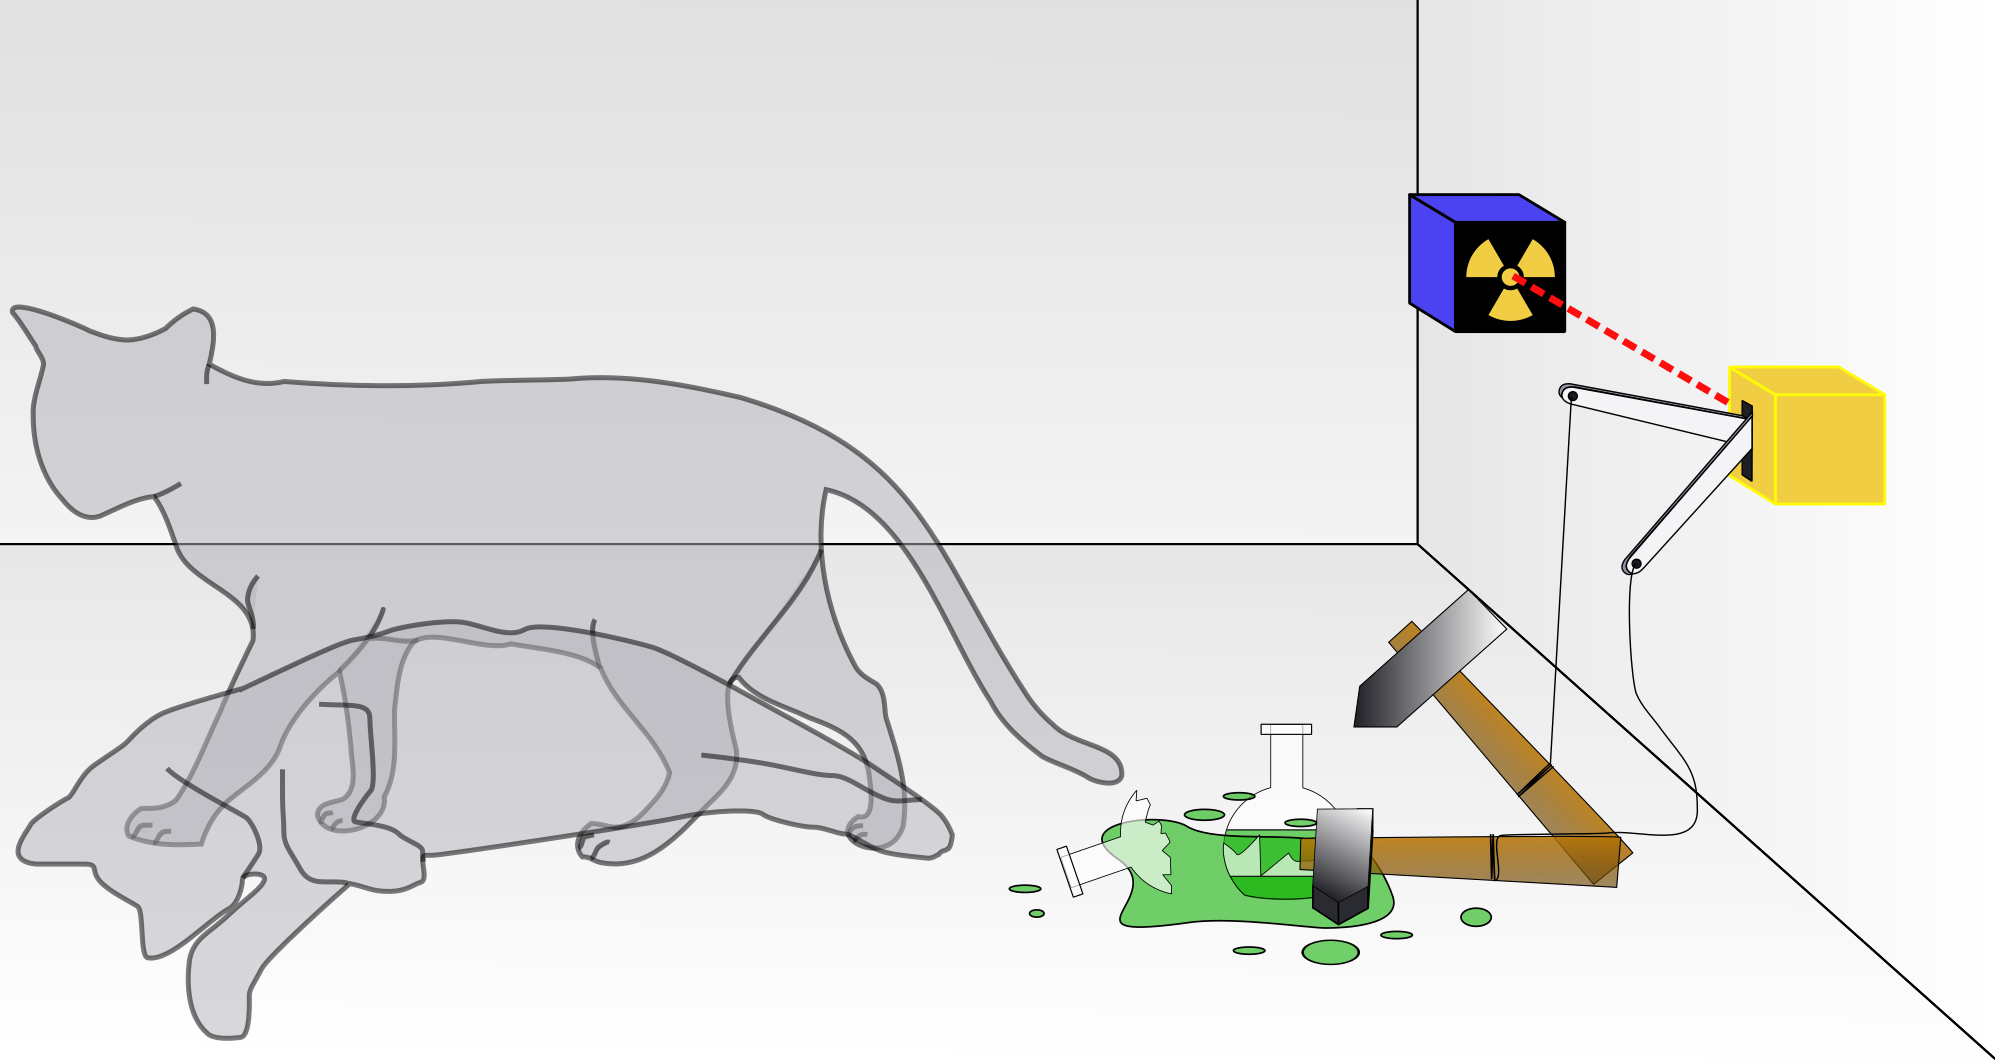
\includegraphics[width=100mm]{Chapter03/Schrodingers_cat.png}
  \caption[Caption for LOF]{A depiction of Schr\"{o}dinger's cat being both dead and alive.\protect\footnotemark}
  \label{deadlivecat}
  \end{figure}
  \footnotetext{ Original by Dhatfield. This image is licensed under the Creative Commons Attribution-Share Alike 3.0 Unported license. Source: https://commons.wikimedia.org/wiki/File:Schrodingers\_cat.svg}
  Such a distribution arises in this context because initially there is an atom that is in a superposition of decayed and non-decayed states, and so the expectation of $\hat{T}^{\mu\nu}(y)$ will have non-zero components both in the location where the non-decayed atom would be, and also in the locations of the decayed atom and the particle the atom emitted. As the decayed atom part of the state interacts with the poison releasing device, this device will also enter into a superposition so that in both the location of the poison containing flask and in the locations of all the poison atoms in the container containing the cat and into which the poison is released, the expectation of $\hat{T}^{\mu\nu}(y)$ will have non-zero components. And then the cat will enter into a superposition of being in a dead state and an alive state, and so that the expectation of $\hat{T}^{\mu\nu}(y)$ will have non-zero components in locations where the dead cat ends up and where the living cat happens to be. So the expectation of $\hat{T}^{\mu\nu}(y)$ in the locations of the container containing the cat will be very different from what someone would actually observe.


  To overcome this defect, information about the mass-energy density on $S$ is used, specifically the values of $\tau_S(x)$ for $x\in S^1(y)$ where  $S^1(y)$ is defined to consist of all the spacetime locations of $S$ outside the light cone of $y$ as depicted in figure \ref{S2}.  

 \begin{figure}[ht!]
\captionsetup{justification=justified}
\centering

\tikzmath{
\a= 1;  
\e = 0.1;
\h=-1;
\hae=(3*\a*\a+6*\a*\e+7*\e*\e-3*\a*sqrt(\a*\a+4*\e*\e)-4*\e*sqrt(\a*\a+4\e*\e))/(4*\a+4*\e-2*sqrt(\a*\a+4*\e*\e));
\hae=0.0463647;
\hae=0.0858615;
\circsize=1.2;
\md = (\a+\h)/2;
\lrange = 4;
\rrange=2;
\ss=(-\lrange-\a)/2;
\sss=\a+(\rrange-\a)/2;
\tlen=0.75;
\labelpos=(-\lrange-\a)/2;
} 

\begin{tikzpicture}[thick, scale=2]

\def\dotsize{0.7}

\definecolor{tempcolor}{RGB}{0,151,76}
\draw[<->] (-\lrange, \h) node[left] {$S_0$} -- (\rrange, \h) node[right] {$S_0$};
\filldraw (0,0) circle (\dotsize pt) node [below right] {$y$} ;
              


\draw[<-] (-\lrange, \a)  -- (-\a, \a)  {};
\draw[gray, dotted] (-\a, \a) -- (0,0) {};
\draw[gray, dotted](0,0) -- (\a, \a) {};
\draw[->](\a, \a) --  (\rrange, \a)  ;         
\coordinate (B) at (\a,\a);
\node at (B)[red,circle,fill,inner sep=\circsize pt]{};
\coordinate (A) at (-\a,\a);
\node at (A)[red,circle,fill,inner sep=\circsize pt]{};
\coordinate (C) at (0,0);
\node at (C)[black,circle,fill,inner sep=\circsize pt]{};



\coordinate[label = above:$S^1(y)$]  (D) at (\ss,\a);
\coordinate[label = above:$S^1(y)$]  (D) at (\sss,\a);

\draw[->] (\rrange,\md-\tlen/2) --  (\rrange,\md+\tlen/2) node[midway,right]{time}; 
 
\node (start) at (\labelpos,\h) [below] {Initial State $\ket{\Psi_0}$};
\node (evolution) at (\labelpos,\md+0.05) [below] {Unitary Evolution $U_{S'S_0}\ket{\Psi_0}$};
\node (final) at (\labelpos,\a) [below] {Unitary Evolution $U_{SS_0}\ket{\Psi_0}$};
%\node at (-\ss+0.17,\mn-0.18){$-a_0$};
\draw [->, shorten <= 5pt] (start) [above] -- (evolution); 
\draw [->] (evolution) -- (final); 
\end{tikzpicture}

\vspace*{2px}
\caption{The set $S^1(y)$ consists of all the spacetime locations of $S$ outside the light cone of $y$. The $T^{\mu\nu}(y)$-beables are calculated using the initial state $\ket{\Psi_0}$ together with the values of $\tau_S(x)$ for $x\in S^1(y)$. }
\label{S2}
\end{figure}
So in the case of Schr\"{o}dinger's cat, if the cat were dead,  light reflecting off the dead cat and going off into outer space would eventually intersect the spacelike hypersurface $S$, and the light distribution on $S$ would register the inanimate status of the cat. On the other hand, if the cat were alive, the light reflecting off the living cat and going off into outer space would also intersect $S$, but now the light distribution on $S$ would register the different locations the living cat was in as it moved about. Because light travels at a constant speed in a vacuum, the state of the cat at earlier times would be described by light distributions in regions on $S$ that were further away from the cat than those light distributions in regions of $S$ that described the cat in more recent times. 

Now if the cat was in a superposition of dead and alive states, then assuming there is no intermediate collapse of the global quantum state,  the spacelike hypersurface $S$ would also enter into a superposition of different states corresponding to these different distributions of light registered on $S$. But if a notional measurement on $S$ is made that determines which of these distributions is actually realized on $S$, then this determination will determine which history was actualized, and hence determine whether the cat actually survived Schr\"{o}dinger's experiment or whether it perished. Thus, by conditioning on one of these two distributions on $S$ being actualized, the conditional expectation of the stress-energy tensor in the vicinity of where Schr\"{o}dinger's cat might be 
will not describe a situation like the one depicted in figure \ref{deadlivecat}.   Rather, it will either describe a situation like the one depicted in figure \ref{livecat}, or it will describe a situation like the one depicted in figure \ref{deadcat}. Which of these two situations occur will be determined by whether the measurement outcome on $S$ corresponds to a light distribution reflected from a living cat, or to a light distribution reflected from a dead cat. 
\begin{figure}[ht!]
  \captionsetup{justification=justified}
  \centering
  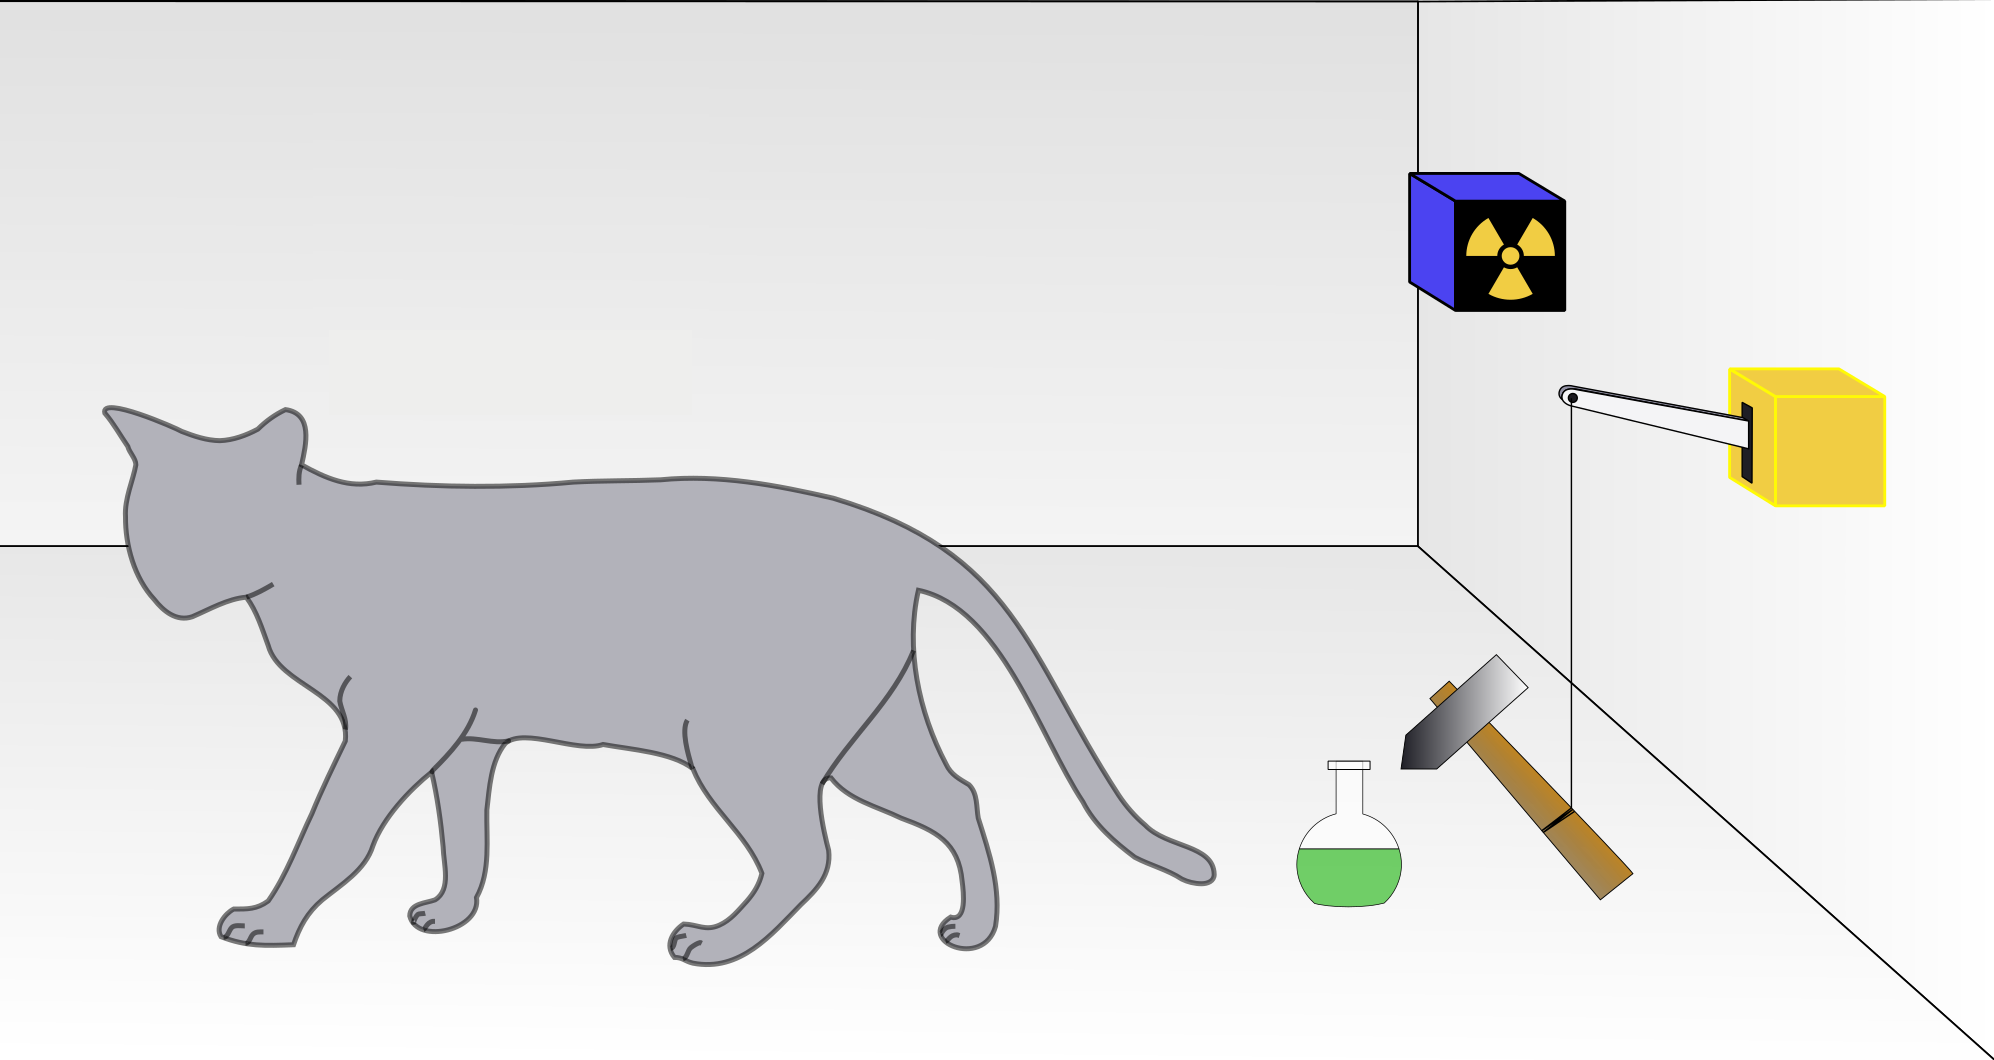
\includegraphics[width=100mm]{Chapter03/Schrodingers_livecat.png}
  \caption[Caption for LOF]{A depiction of Schr\"{o}dinger's cat being alive.\protect\footnotemark}
  \label{livecat}
  \end{figure}
  \footnotetext{ Original by Dhatfield. This image is licensed under the Creative Commons Attribution-Share Alike 3.0 Unported license. Source: https://upload.wikimedia.org/wikipedia/commons/archive/9/91/20080627113554!Schrodingers\_cat.svg}

  \begin{figure}[ht!]
    \captionsetup{justification=justified}
    \centering
    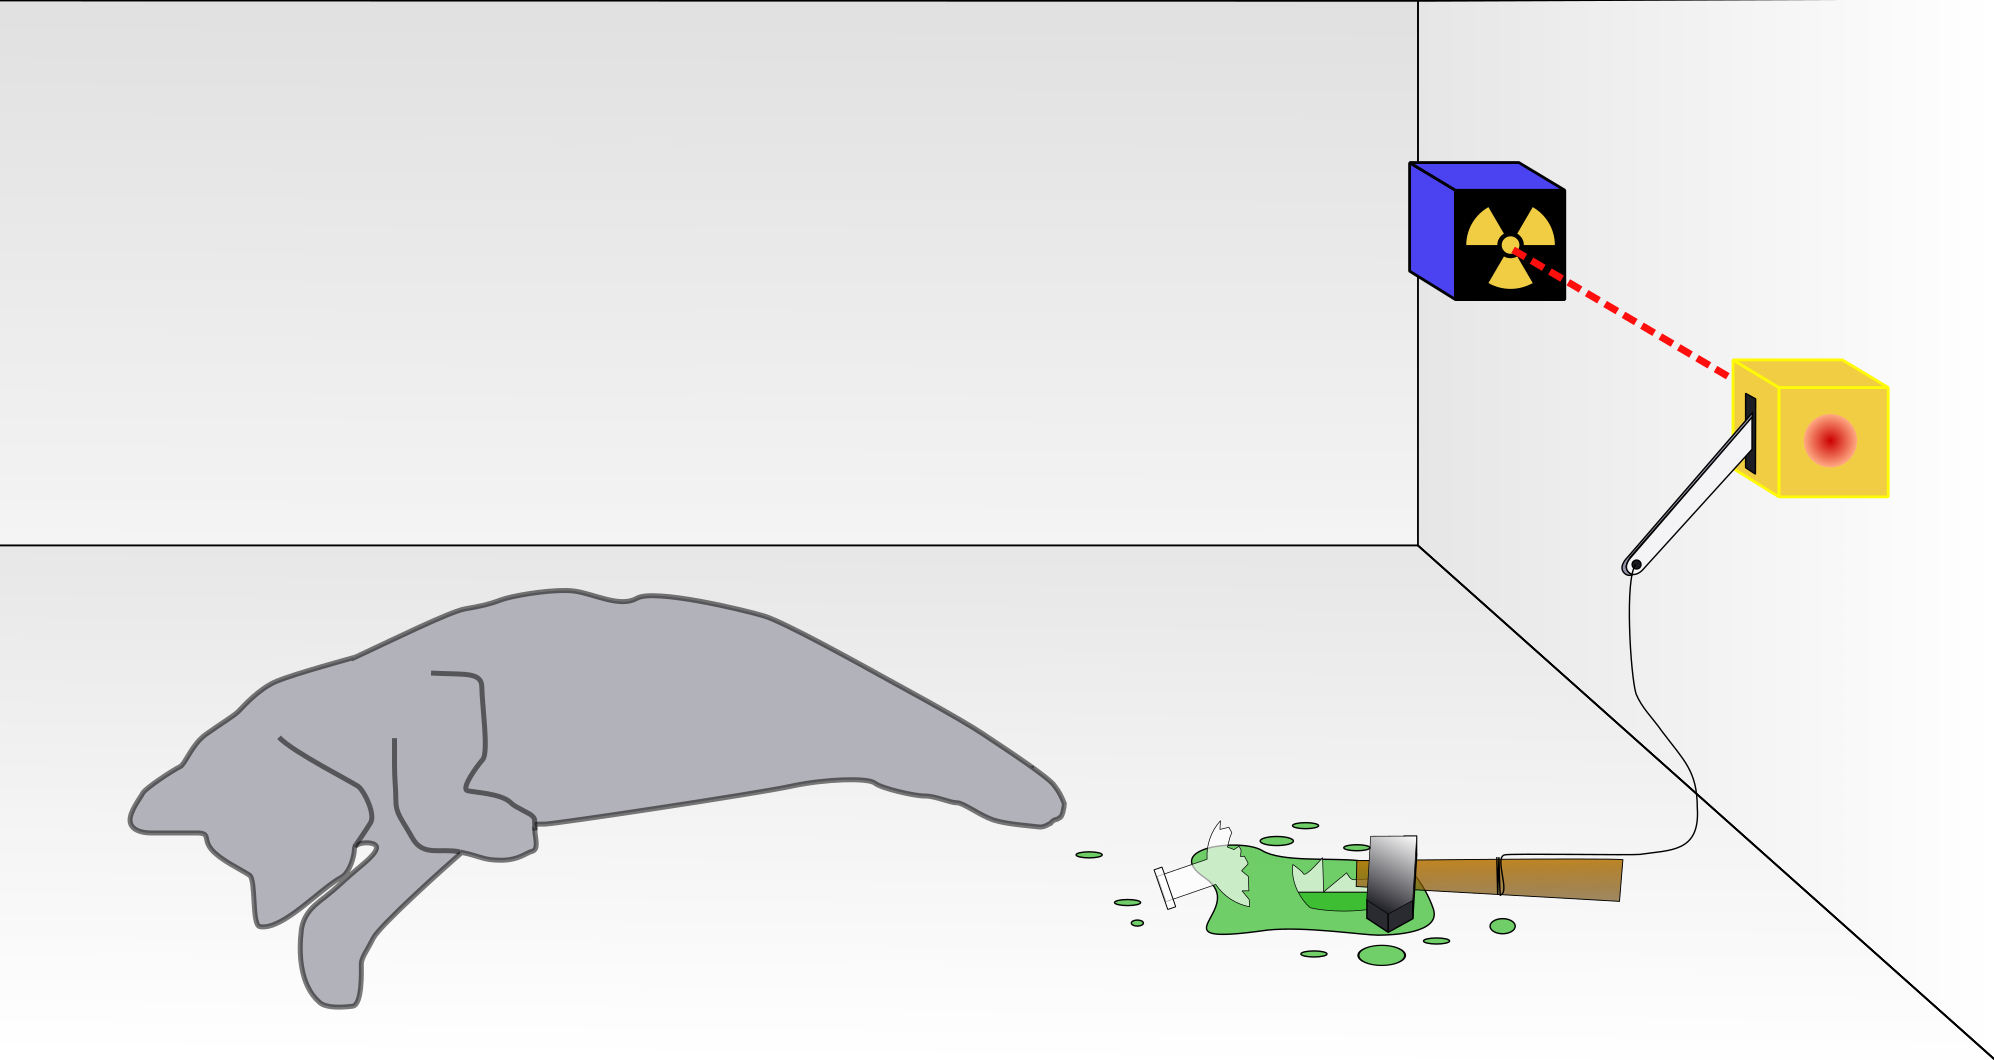
\includegraphics[width=100mm]{Chapter03/Schrodingers_deadcat.png}
    \caption[Caption for LOF]{A depiction of Schr\"{o}dinger's cat being dead.\protect\footnotemark}
    \label{deadcat}
    \end{figure}
    \footnotetext{ Original by Dhatfield. Altered by removing numbers and making into two separate figures. This image is licensed under the Creative Commons Attribution-Share Alike 3.0 Unported license. Source: https://upload.wikimedia.org/wikipedia/commons/archive/9/91/20080627113554!Schrodingers\_cat.svg}

\section{Calculating Kent's $T^{\mu\nu}(y)$-beables \label{kentcalculation}}
Having given a qualitative description in the last section of how a measurement outcome on $S$ determines which facts obtain in reality such as whether Schr\"{o}dinger's cat is alive or dead, we now give a more quantitative description of how Kent's beables are calculated. Kent's beables specify $T^{\mu\nu}(y)$ values for all $y$ between $S_0$ and $S$, and for all $\mu,\nu = 0, 1, 2,$ and $3$. Kent's $T^{\mu\nu}(y)$-beables are conditional expectation values, and the conditional expectation that we need to calculate depends on the notion of \textbf{conditional probability}\index{conditional probability}. In probability theory, the conditional probability $P(q|r)$ that a statement $q$ is true given that a statement $r$ is true is given by the formula
\begin{equation} \label{conditionalprobability}
  P(q|r)=\frac{P(q\, \&\,  r)}{P(r)}. 
\end{equation}
If we now define $q(\tau)$ to be the statement that some quantity $T$  takes the value $\tau$, then the  \textbf{conditional expectation}\index{conditional expectation} of  $T$ given $r$ will be given by the formula
\begin{equation}\label{conditionalexpectation}
\ev*{T}_r\myeq\sum_\tau P(q(\tau)|r)\tau
\end{equation}
where the summation is over all the possible values $\tau$ that $T$ can take.

We thus define Kent's $T^{\mu\nu}(y)$-beable to be $\ev*{T^{\mu\nu}(y)}_{\tau_S}\myeq \ev*{T^{\mu\nu}(y)}_{r(\tau_S,y)}$\label{Kentbeable} where $r(\tau_S, y)$ is the statement that $T_S(x)$ has the determinate value $\tau_S(x)$ for all $x\in S^1(y)$, and where $q(\tau)$ in equation (\ref{conditionalexpectation}) is the statement that $T^{\mu\nu}(y)$ (understood in the conventional non-Kentian sense) takes the value $\tau$. It is these $T^{\mu\nu}(y)$-beables $\ev*{T^{\mu\nu}(y)}_{\tau_S}$ that give a one-world picture of reality in Kent's theory. 

We can see how the formula (\ref{conditionalexpectation}) relates to the Sch\"{o}dinger's cat scenario. The distribution of light reflected off the cat that intersects $S^1(y)$ when ``measured'' will determine a definite statement $r(\tau_S, y)$ about the mass-energy density on $S^1(y)$. This in turn will determine the range of $\tau$ for which $P(q(\tau)|r(\tau_S,y))$ is not close to zero, and hence where the stress-energy distribution $\ev*{T^{\mu\nu}(y)}_{\tau_S}$ is not zero. This stress-energy distribution will then correspond either to that of  a living cat or to that of a dead cat, but not both.  

 Coming back to the question of why we don't include any information about $\tau_S(x)$ for $x\in S$ from within the light cone of $y$, we need to consider in more detail how we would calculate $\ev*{T^{\mu\nu}(y)}_{\tau_S}$. From (\ref{conditionalprobability}) and (\ref{conditionalexpectation}), we will be able to perform this calculation so long as we can calculate $P(q(\tau) \, \&\,  r(\tau_S,y))$ and $P(r(\tau_S,y))$. 
 
 Calculating $P(r(\tau_S,y))$ is relatively straightforward. As described on page \pageref{simultaneous}, we can find an orthonormal basis $\{\ket*{\Psi^{(i)}}:i\}$ of $H_S$ consisting of simultaneous $\hat{T}_S$-eigenstates and simultaneous $\hat{T}_S$-eigenvalues $\tau^{(i)}_S$ respectively. The probability $P(r(\tau_S,y))$ will then be  
 \begin{equation}\label{rProb}
 P(r(\tau_S,y))=\sum_{\substack{i \text{ such that} \\ \tau_S^{(i)}(x)=\tau_S(x)\\ \text{ for all }x\in S^1(y)}}\abs{\mel{\Psi^{(i)}}{U_{SS_0}}{\Psi_0}}^2
 \end{equation} where we have used equation (\ref{bornpsi}).

 But calculating $P(q(\tau) \, \&\,  r(\tau_S,y))$ is a bit more involved because in the Tomonaga-Schwinger picture, the definition of observables via 
 \begin{equation}\tag{\ref{tsobservable} revisted}
  \hat{O}(x)=U[S]\hat{\bm{O}}(x)U[S]^{-1}
\end{equation}
requires that $x\in S$.
This means that we can't define $\hat{T}^{\mu\nu}(y)$ according to (\ref{tsobservable}) since $y\not\in S$.\footnote{If we did attempt to use (\ref{tsobservable}) to define $\hat{T}^{\mu\nu}(y)=U[S]\hat{\bm{T}}^{{\mu\nu}}(y)U[S]^{-1}$, then $\hat{T}^{\mu\nu}(y)$ would have a (non-local) dependence on $S$, and such a dependence would not be desirable.} However, we do not face such restrictions in the Heisenberg picture, so one approach would be to calculate $P(q(\tau) \, \&\,  r(\tau_S,y))$ in the Heisenberg picture. As we will see in section \ref{kentinterpretationconsistency}, this is not the approach that Kent takes, but nevertheless, in the Heisenberg picture, it is easier to see why we don't include information from $S$ within the light cone (without begging the question of why we don't) when calculating $P(q(\tau) \, \&\,  r(\tau_S,y))$. To see why this is so, consider the simpler case of just two measurable quantities ${F}$ and ${G}$ which we assume to have a discrete range of possible values and for which we wish to calculate the joint probability $P((F=f)\, \&\, (G=g))$. To do this in the Heisenberg picture, we need an orthonormal basis of the state space $\{\ket*{\Phi^{(i)}}:i\}$ consisting of simultaneous eigenstate of the observables $\hat{\bm{F}}$ and $\hat{\bm{G}}$ with eigenvalues $f^{(i)}$ and $g^{(i)}$ respectively so that $\hat{\bm{F}}\ket*{\Phi^{(i)}}=f^{(i)}\ket*{\Phi^{(i)}}$ and $\hat{\bm{G}}\ket*{\Phi^{(i)}}=g^{(i)}\ket*{\Phi^{(i)}}$, and when the system is in the state $\ket*{\Phi^{(i)}}$, the quantity $F$ will have the value $f^{(i)}$, and the quantity $G$ will have the value $g^{(i)}$. Given that the system is in the state $\ket*{\Phi}$, the joint probability $P((F=f)\, \&\, (G=g))$ can then be calculated using the Born rule to get
$$P((F=f)\, \&\, (G=g))=\sum_{\substack{i \text{ such that} \\ f^{(i)}=f \text{ and } g^{(i)}=g}}\abs{\ip{\Phi^{(i)}}{\Phi}}^2.$$
But  in order for such an orthonormal basis to exist, it is necessary that $\hat{F}$ and $\hat{G}$ commute.\footnote{This is because given such an orthonormal basis $\{\ket*{\Phi^{(i)}}:i\}$ of simultaneous eigenstates of $\hat{\bm{F}}$ and $\hat{\bm{G}}$, we have 
$$\hat{\bm{F}}\hat{\bm{G}}\ket*{\Phi^{(i)}}=f^{(i)}g^{(i)}\ket*{\Phi^{(i)}}=g^{(i)}f^{(i)}\ket*{\Phi^{(i)}}=\hat{\bm{G}}\hat{\bm{F}}\ket*{\Phi^{(i)}}$$ so for any arbitrary state $\ket*{\Phi}=\sum_i c_i \ket*{\Phi^{(i)}},$ we have 
$$\hat{\bm{F}}\hat{\bm{G}}\ket*{\Phi}=\sum_i c_i \hat{\bm{F}}\hat{\bm{G}}\ket*{\Phi^{(i)}}= \sum_i c_i \hat{\bm{G}}\hat{\bm{F}}\ket*{\Phi^{(i)}}=\hat{\bm{G}}\hat{\bm{F}}\ket*{\Phi}.$$ 
} This means that if $\hat{F}$ and $\hat{G}$ do not commute, then we cannot define the joint probability $P((F=f)\, \&\, (G=g)).$

Now quantum field theory is so constructed that $\hat{\bm{T}}^{{00}}(x)$ and $\hat{\bm{T}}^{{\mu\nu}}(y)$ will not commute when $x$ and $y$ are not spacelike separated, but $\hat{\bm{T}}^{{\mu'\nu'}}(x)$ and $\hat{\bm{T}}^{{\mu\nu}}(y)$ will commute when $x$ and $y$ are spacelike separated.\footnote{The proof of this statement need not concern us, but one can see that this is the case by considering the four potential commutation relations and the decomposition of the stress-energy tensors as in terms of the four-potentials  -- see \cite[p. 1443--1444]{SchwingerJulianI}.} As we will see on page \pageref{TSdef}, $T_S(x)$ will have a $T^{00}(x)$ component, and so we can only be sure that $\hat{\bm{T}}_S(x)$ will commute with  $\hat{\bm{T}}^{{\mu\nu}}(y)$ if $x$ and $y$ are spacelike separated. In other words, $\hat{\bm{T}}_S(x)$ and $\hat{\bm{T}}^{{\mu\nu}}(y)$ will commute if $x$ is outside the light cone of $y$. Extending this argument to multiple $x\in S$, we see that we can only guarantee that the conditional expectation of $T^{\mu\nu}(y)$ is definable if we restrict our conditioning on the value of $T_S(x)$ to $x\in S^1(y)$, that is, to $x$ in $S$ outside the light cone of $y$.

Having explained why we don't include any information about $\tau_S(x)$ for $x\in S$ from within the light cone of $y$, we can now proceed to calculate  $P(q(\tau) \, \&\,  r(\tau_S,y))$. Now although there is no spacelike hypersurface that contains both $y$ and $S^1(y)$, we can find a sequence of spacelike hypersurfaces $S_n(y)$ such that\label{siydef} $S_n(y)\subset S_{n'}(y)$ for $n<n'$, and such that for any $x\in S^1(y)$, there exists $n$ such that $x\in S_n(y)$. An example of one such $S_n(y)$ is shown in figure \ref{S3}. When there is no ambiguity, we will drop the $y$ and write $S_n$ instead of $S_n(y)$. 

 \begin{figure}[ht!]
\captionsetup{justification=justified}
\centering

\tikzmath{
\a= 1;  
\e = 0.1;
\lam=0.9;
\h=-1;
\hae=(3*\a*\a+6*\a*\e+7*\e*\e-3*\a*sqrt(\a*\a+4*\e*\e)-4*\e*sqrt(\a*\a+4\e*\e))/(4*\a+4*\e-2*sqrt(\a*\a+4*\e*\e));
\hae=0.205678;
\circsize=1.2;
\md = (\a+\h)/2;
\lrange = 4;
\rrange=2;
\fictlabel=(\rrange-\lrange)/2;
\ss=(-\lrange-\a)/2;
\sss=\a+(\rrange-\a)/2;
\tlen=0.75;
\labelpos=(-\lrange-\a)/2;
} 

\begin{tikzpicture}[thick, scale=2]

\def\dotsize{0.7}

\definecolor{tempcolor}{RGB}{0,151,76}
\draw[<->] (-\lrange, \h) node[left] {$S_0$} -- (\rrange, \h) node[right] {$S_0$};
\filldraw (0,0) circle (\dotsize pt) node [below right] {$y$} ;
              
\draw[->] (\rrange,\md-\tlen/2) --  (\rrange,\md+\tlen/2) node[midway,right]{time}; 

\draw[->,blue, thick] [domain=-\a/2:-\lrange, samples=150]   plot (\x, {\a-\e/2-1/2*(sqrt(\lam*\lam*pow(\x+\hae+\a,2)+\e*\e)-\e+\lam*(\x+\hae+\a))}) node[left, black]{$S_n(y)$}  ;
\draw[blue, thick] [domain=-\a/2:\a/2, samples=150] plot (\x, {sqrt(\lam*\lam*\x*\x+\e*\e)-\e})   node[right, black]{$S_n(y)$};
\draw[->,blue, thick] [domain=\a/2:\rrange, samples=150]   plot (\x, {\a-\e/2-1/2*(sqrt(\lam*\lam*pow(\x-\hae-\a,2)+\e*\e)-\e-\lam*(\x-\hae-\a))}) node[right, black]{$S_n(y)$}  ;
\draw[gray] (-\lrange, \a)  -- (\rrange, \a)  {};
\draw[gray, dashed] (-\a, \a) -- (0,0) {};
\draw[gray, dashed](0,0) -- (\a, \a) {};
\draw[gray](\a, \a) --  (\rrange, \a)  ;         
\coordinate (B) at (\a,\a);
\node at (B)[red,circle,fill,inner sep=\circsize pt]{};
\coordinate (A) at (-\a,\a);
\node at (A)[red,circle,fill,inner sep=\circsize pt]{};
\coordinate (C) at (0,0);
\node at (C)[black,circle,fill,inner sep=\circsize pt]{};

\coordinate[label = above:$S$]  (D) at (0,\a);

\coordinate[label = above:$S$]  (D) at (\sss,\a);

\filldraw (\ss,\a) circle (\dotsize pt) node [above] {$x\in S_n(y)\cap S$} ;


 
\node (start) at (\labelpos,\h) [below] {Initial State $\ket{\Psi_0}$};
\node (evolution) at (\labelpos,\md+0.05) [below] {Unitary Evolution $U_{S_nS_0}\ket{\Psi_0}$};
\node (final) at (\labelpos,\a) [below] {Unitary Evolution $U_{SS_0}\ket{\Psi_0}$};
%\node at (-\ss+0.17,\mn-0.18){$-a_0$};
\draw [->, shorten <= 5pt] (start) [above] -- (evolution); 
\draw [->] (evolution) -- (final); 
\end{tikzpicture}

\vspace*{2px}
\caption{$S_n\myeq S_n(y)$ is a spacelike hypersurface containing $y$ and all of $S^1(y)$ in the limit as $n\rightarrow\infty$.   }
\label{S3}
\end{figure}
Such a sequence $S_n$ of hypersurfaces will be sufficient to calculate  $P(q(\tau) \, \&\,  r(\tau_S,y))$. So let us define $r_n$ to be the statement that  $T_S(x)$ has the determinate value $\tau_S(x)$ for all $x\in S_n\cap S$. We recall that in the Tomonaga-Schwinger formulation of relativistic quantum physics, the operators $\hat{T}_S(x)$ and $\hat{T}^{\mu\nu}(y)$ for fixed $\mu,\nu$ commute when $x$ and $y$ are spacelike-separated. It therefore follows that we can express any state of $H_{S_n}$ as a superposition of simultaneous eigenstates of $\hat{T}^{\mu\nu}(y)$ and $\hat{T}_S(x)$ for $x\in S_n\cap S$.\footnote{We make the same approximation as mentioned on page \pageref{simultaneous} in footnote \ref{glosssim}.}  For a particular choice of $\mu,\nu$, we can then form an orthonormal basis $\{\ket*{\Psi_{n}^{(i)}}:i\}$ of $H_{S_n}$ consisting of simultaneous $\hat{T}^{\mu\nu}(y)$, $\hat{T}_S(x)$-eigenstates so that $\hat{T}^{\mu\nu}(y)\ket*{\Psi_{n}^{(i)}}=\tau^{(i)}\ket*{\Psi_{n}^{(i)}}$ and $\hat{T}_{S}(x)\ket*{\Psi_{n}^{(i)}}=\tau_S^{(i)}(x)\ket*{\Psi_{n}^{(i)}}$ for $x\in S_n\cap S$, where $\tau^{(i)}$ and $\tau_S^{(i)}(x)$ are the corresponding eigenvalues. The probability $P(q(\tau) \, \&\,  r_n)$ will then be
$$P(q(\tau) \, \&\,  r_n) =\sum_{\substack{i \text{ such that } \tau^{(i)}=\tau \\ \text{and }\tau_S^{(i)}(x)=\tau_S(x)\\ \text{ for all }x\in S_n\\ }}\abs{\mel{\Psi_n^{(i)}}{U_{SS_0}}{\Psi_0}}^2.$$
Taking the limit as $n$ tends to infinity, we can calculate the probability $P(q(\tau) \, \&\,  r(\tau_S,y))$ to be
\begin{equation}\label{qrProb}
P(q(\tau) \, \&\,  r(\tau_S,y))=\lim_{n\rightarrow\infty}P(q(\tau) \, \&\,  r_n).
\end{equation}
Plugging (\ref{rProb}) and (\ref{qrProb}) into (\ref{conditionalprobability}), we can calculate the conditional probability $P(q(\tau) | r(\tau_S,y))$,  and hence the conditional expectation  $\ev*{T^{\mu\nu}(y)}_{\tau_S}\myeq \ev*{T^{\mu\nu}(y)}_{r(\tau_S,y)}$ via equation (\ref{conditionalexpectation}).
In section \ref{kentinterpretationconsistency}, we will give a more detailed description of this calculation in order to show that the predictions Kent's theory makes are consistent with standard quantum physics.
 
 
\section{Kent's toy example}\label{toysection}
To get a feel for how all the elements of Kent's theory fit together, we will conclude this chapter by describing Kent's toy model example that he discusses in his 2014 paper.\footnote{See \cite[p. 3--4]{Kent2014}.} In his toy model, Kent considers a system in one spatial dimension which is the superposition of two localized states/wave functions\footnote{So far in this chapter, we have been describing systems in terms of their quantum states rather than their \textbf{quantum wave functions}\index{quantum wave functions}. It is easiest to understand what a quantum wave function is in the context of a single particle system. In the Schr\"{o}dinger picture, a particle in state $\ket*{\psi(t)}$ allows us to calculate the expectation value of a quantity $O$ belonging to the particle via the formula $\ev{\hat{\bm{O}}}{\psi(t)}$ where $\hat{\bm{O}}$ is the observable corresponding to $O$. One such quantity is the particle's spatial location. If the particle is at spatial location $\bm{x}$, then the particle will be in the state $\ket*{\bm{x}}$ (c.f. the definition of $\ket*{x}$ in footnote \ref{ketx} on page \pageref{ketx}.) where the position observable $\hat{\bm{X}_i}$ satisfies $\hat{\bm{X}_i}\ket*{\bm{x}}=x_i\ket*{\bm{x}}$ for $i=1,2$, or $3$. The corresponding wave function for this particle is then   $\psi(\bm{x}, t)=\ip*{\bm{x}}{\psi(t)}$. For a particle restricted to one spatial dimension, the particle would have a wave function $\psi(z, t)=\ip*{z}{\psi(t)}$ where $z$ is now just a single number that specifies the particle's possible position. We will write $\psi$ to denote the wave function itself, and $\psi(z,t)$ to denote the value of the wave function $\psi$ at spacetime location $(z,t)$.}  $\psi_0^\text{sys}=c_1 \psi_1^\text{sys}+c_2\psi_2^\text{sys}$ where $\psi_1^\text{sys}$ is localized at spatial location $z_1$, $\psi_2^\text{sys}$ is localized at spatial location $z_2$, and $\abs{c_1}^2+\abs{c_2}^2=1$. According to the Copenhagen interpretation, a measurement on this system would collapse the wave function of $\psi_0^\text{sys}$ to the wave function of $\psi_1^\text{sys}$ with probability $\abs{c_1}^2$, and to the wave function of $\psi_2^\text{sys}$ with probability $\abs{c_2}^2$. The purpose of Kent's toy model is to show that within his interpretation, there is something analogous to wave function collapse.  In order for this ``collapse'' to happen, one needs to consider how the system interacts with light. Thus, Kent supposes that a photon (which is modelled as a point particle) comes in from the left, and as it interacts with the two states $\psi_1^\text{sys}$ and $\psi_2^\text{sys}$, the photon enters into a superposition of states, corresponding to whether the photon reflects off the localized $\psi_1^\text{sys}$-state at time $t_1$ or the localized $\psi_2^\text{sys}$-state at time $t_2$. The photon in superposition then travels to the left and eventually reaches the one dimensional spacelike hypersurface $S$ at locations $\gamma_1$ and $\gamma_2$ as shown in figure  \ref{TM1}.

 \begin{figure}[ht!]
\captionsetup{justification=justified}
\centering
\tikzmath{
\a=5.3;  
\psione=0;
\psitwo=1;
\e = 0.1;
\h=-0.8;
\phstartx=-2.9;
\phstarty=-.8;
\tbeg=\phstarty;
\ca=\phstartx-\tbeg;
\ttwo=\psitwo-\ca;
\cb=\ttwo+\ca;
\xend=\ttwo-\a+\cb;
\tone=\psione-\ca;
\cc=\tone+\ca;
\xendz=\tone-\a+\cc;
\tthree=\cc+\tone-\psitwo;
\circsize=0.05;
\md = (\a+\h)/2;
\tlen=0.75;
\textscale = 0.8;
\picscale = 0.95;
\nudge=0.1;
\tnudge=(\ttwo-\tone)/2;
\ttesta=2*\tone-\ttwo-\tnudge;
\ttestb=2*\tone-\ttwo+\tnudge;
\ttestc=\ttwo-\tnudge;
\ttestd=\ttwo+\tnudge;
\sonea=\a+\psione-\ttesta;
\sadd=0.5;
\lrange = -(\psione-\a+\ttesta)+\sadd;
\rrange =\a+\psitwo-\ttesta+\sadd; 
\timex=\rrange-0.7;
} 
\begin{tikzpicture}[scale=1.2,
declare function={
	testxonep(\ps,\t)=\a+\ps-\t;
	testxonem(\ps,\t)=\ps-\a+\t; 
},
 ] 

\definecolor{tempcolor}{RGB}{250,190,0}
\definecolor{darkgreen}{RGB}{40,190,40}
\draw[<->] (-\lrange, \h) node[left, scale=\textscale] {$S_0$} -- (\rrange, \h) node[right, scale=\textscale] {$S_0$};
\draw[<->] (-\lrange, \a) node[left, scale=\textscale] {$S$} -- (\rrange, \a) node[right, scale=\textscale] {$S$};

              
\draw[->, shorten <= 5pt,  shorten >= 1pt] (\psione,\h) node[below, scale=\textscale]{$\psi_1^{\text{sys}}$} node[above left, scale=\textscale]{$Z=z_1$}-- (\psione,\a);
\draw[->,  shorten <= 5pt,  shorten >= 1pt] (\psitwo,\h) node[below, scale=\textscale]{$\psi_2^{\text{sys}}$} node[above right, scale=\textscale]{$Z=z_2$}-- (\psitwo,\a);

\draw[dashed, tempcolor, ultra thick](\phstartx,\tbeg) node[below left=-2,scale=\textscale]{}--(\psitwo,\ttwo ) node[above, pos=0.3, rotate=45,scale=0.7,black] {$Z=c(t-t_1)+z_1$} node[below, pos=0.3, rotate=45,scale=0.7,black] {photon};
\draw[dashed, tempcolor, ultra thick](\psitwo,\ttwo)--(\xend,\a) node[above, pos=0.48, rotate=-45,scale=0.7,black] {$Z=c(t_2-t)+z_2$} ;
\draw[dashed, tempcolor, ultra thick](\psione,\tone)--(\xendz,\a)node[above, pos=0.45, rotate=-45,scale=0.7,black] {$Z=c(t_1-t)+z_1$} ;

\draw [black,fill] (\xendz,\a) circle [radius=\circsize] node [black,above,scale=\textscale] {$\gamma_1$}; 
\draw [black,fill] (\xend,\a) circle [radius=\circsize] node [black,above,scale=\textscale] {$\gamma_2$}; 
%\draw[dashed, darkgreen, ultra thick](\psione,\tone)--(\psitwo,\tthree);
%\draw [black,fill] (\psitwo,\tthree) circle [radius=\circsize] node [black,below=4,right,scale=\textscale] {$t=2t_1-t_2$}; 


\draw [black,fill] (\psione,\tone) circle [radius=\circsize] node [black,left=4,scale=\textscale] {$t_1$}; 
\draw [black,fill](\psitwo,\ttwo)circle [radius=\circsize] node [black,right,scale=\textscale, align=left] {$t_2=t_1+\frac{z_2-z_1}{c}$.}; 

%\draw [decorate, decoration = {calligraphic brace}] (\psitwo+\nudge,\ttwo) --  (\psitwo+\nudge,\tone+\nudge/4) node[midway,right, scale=\textscale]{$t_2-t_1$}; 
%\draw [decorate, decoration = {calligraphic brace}] (\psitwo+\nudge,\tone-\nudge/4) --  (\psitwo+\nudge,2*\tone-\ttwo) node[midway,right, scale=\textscale]{$t_2-t_1$}; 

\draw[->] (\timex,\md-\tlen/2) --  (\timex,\md+\tlen/2) node[midway,right, scale=\textscale]{time}; 
 
%\draw[dotted](\psione,\ttesta)--({testxonep(\psione,\ttesta)},\a);
%\draw[dotted](\psione,\ttesta)--({testxonem(\psione,\ttesta)},\a);
%\draw [black,fill](\psione,\ttesta) circle [radius=\circsize] node [black,below=5,right,scale=\textscale] {$y_a$}; 

%\draw[magenta,->,ultra thick] ({testxonem(\psione,\ttesta)},\a)--(-\lrange,\a);
%\draw[magenta,->,ultra thick] ({testxonep(\psione,\ttesta)},\a)--(\rrange,\a);

\end{tikzpicture}% pic 1

\vspace*{2px}
\caption{Kent's toy model}
\label{TM1}
\end{figure}
We now suppose that when the mass-energy density $S$ is ``measured'', the energy of the photon is found to be at $\gamma_1$ rather than at $\gamma_2$. We then consider the mass-density at early spacetime locations $y^a_1=(z_1,t_a)$ and $y^a_2=(z_2,t_a)$ as shown in figure \ref{TM2} (a) and (b). 
 
 
  \begin{figure}[ht!]
\captionsetup{justification=justified}
\centering
\tikzmath{
\a=5.3;  
\psione=0;
\psitwo=1;
\e = 0.1;
\h=-0.8;
\labelx=(\psione+\psitwo)/2;
\labely=-1.5;
\phstartx=-2.9;
\phstarty=-.8;
\tbeg=\phstarty;
\ca=\phstartx-\tbeg;
\ttwo=\psitwo-\ca;
\cb=\ttwo+\ca;
\xend=\ttwo-\a+\cb;
\tone=\psione-\ca;
\cc=\tone+\ca;
\xendz=\tone-\a+\cc;
\tthree=\cc+\tone-\psitwo;
\circsize=0.08;
\md = (\a+\h)/2;
\tlen=0.75;
\textscale = 0.7;
\picscale = 0.58;
\nudge=0.1;
\tnudge=(\ttwo-\tone)/2;
\ttesta=2*\tone-\ttwo-\tnudge;
\ttestb=2*\tone-\ttwo+\tnudge;
\ttestc=\ttwo-\tnudge;
\ttestd=\ttwo+\tnudge;
\sonea=\a+\psione-\ttesta;
\sadd=0.5;
\lrange = -(\psione-\a+\ttesta)+\sadd;
\rrange =\a+\psitwo-\ttesta+\sadd; 
\timex=\rrange-1.5;
} 
\begin{tikzpicture}[scale=\picscale,
declare function={
	testxonep(\ps,\t)=\a+\ps-\t;
	testxonem(\ps,\t)=\ps-\a+\t; 
},
 ] 
\definecolor{tempcolor}{RGB}{250,190,0}
\definecolor{darkgreen}{RGB}{40,190,40}
\draw[<->] (-\lrange, \h) node[left, scale=\textscale] {$S_0$} -- (\rrange, \h) node[right, scale=\textscale] {$S_0$};
\draw[<->] (-\lrange, \a) node[left, scale=\textscale] {$S$} -- (\rrange, \a) node[right, scale=\textscale] {$S$};
              
\draw[->, shorten <= 5pt,  shorten >= 1pt] (\psione,\h) node[below, scale=\textscale]{$\psi_1^{\text{sys}}$} node[above left, scale=\textscale]{$z_1$}-- (\psione,\a);
\coordinate[label = below: (a)]  (D) at (\labelx,\labely); 
\draw[->,  shorten <= 5pt,  shorten >= 1pt] (\psitwo,\h) node[below, scale=\textscale]{$\psi_2^{\text{sys}}$} node[above right, scale=\textscale]{$z_2$}-- (\psitwo,\a);

\draw[dashed, tempcolor, ultra thick](\phstartx,\tbeg) node[below left=-2,scale=\textscale]{}--(\psione,\tone) node[above, pos=0.3, rotate=45,scale=0.7,black] {} node[below, pos=0.3, rotate=45,scale=0.7,black] {};
\draw[dashed, gray](\psione,\tone) node[below left=-2,scale=\textscale]{}--(\psitwo,\ttwo );
\draw[dashed, gray](\psitwo,\ttwo)--(\xend,\a); 
\draw[dashed, tempcolor, ultra thick](\psione,\tone)--(\xendz,\a);

\draw [black,fill] (\xendz,\a) circle [radius=\circsize] node [black,above,scale=\textscale] {$\gamma_1$}; 

\draw[dashed, darkgreen, ultra thick](\psione,\tone)--(\psitwo,\tthree);
\draw [black,fill] (\psitwo,\tthree) circle [radius=\circsize] node [black,below=4,right,scale=\textscale] {$2t_1-t_2$}; 


\draw [black,fill] (\psione,\tone) circle [radius=\circsize] node [black,left=4,scale=\textscale] {$t_1$}; 
\draw [black,fill](\psitwo,\ttwo)circle [radius=\circsize] node [black,above right,scale=\textscale, align=left] {$t_2$}; 

\draw [decorate, decoration = {calligraphic brace}] (\psitwo+\nudge,\ttwo) --  (\psitwo+\nudge,\tone+\nudge/4) node[midway,right, scale=\textscale]{$t_2-t_1$}; 
\draw [decorate, decoration = {calligraphic brace}] (\psitwo+\nudge,\tone-\nudge/4) --  (\psitwo+\nudge,2*\tone-\ttwo) node[midway,right, scale=\textscale]{$t_2-t_1$}; 

\draw[->] (\timex,\md-\tlen/2) --  (\timex,\md+\tlen/2) node[midway,right, scale=\textscale]{time}; 
 
\draw[dotted](\psione,\ttesta)--({testxonep(\psione,\ttesta)},\a);
\draw[dotted](\psione,\ttesta)--({testxonem(\psione,\ttesta)},\a);
\draw [black,fill](\psione,\ttesta) circle [radius=\circsize] node [black,below=5,right,scale=\textscale] {$y^a_1$}; 

\draw[magenta,->,ultra thick] ({testxonem(\psione,\ttesta)},\a)--(-\lrange,\a);
\draw[magenta,->,ultra thick] ({testxonep(\psione,\ttesta)},\a)--(\rrange,\a);

\end{tikzpicture}% pic 1
 % <----------------- SPACE BETWEEN PICTURES
\begin{tikzpicture}[scale=\picscale,  %[x={10.0pt},y={10.0pt}]
declare function={
	testxonep(\ps,\t)=\a+\ps-\t;
	testxonem(\ps,\t)=\ps-\a+\t; 
},
 ] 
\definecolor{tempcolor}{RGB}{250,190,0}
\definecolor{darkgreen}{RGB}{40,190,40}
\draw[<->] (-\lrange, \h) node[left, scale=\textscale] {$S_0$} -- (\rrange, \h) node[right, scale=\textscale] {$S_0$};
\draw[<->] (-\lrange, \a) node[left, scale=\textscale] {$S$} -- (\rrange, \a) node[right, scale=\textscale] {$S$};
              
\draw[->, shorten <= 5pt,  shorten >= 1pt] (\psione,\h) node[below, scale=\textscale]{$\psi_1^{\text{sys}}$} node[above left, scale=\textscale]{$z_1$}-- (\psione,\a);
\coordinate[label = below: (b)]  (D) at (\labelx,\labely); 
\draw[->,  shorten <= 5pt,  shorten >= 1pt] (\psitwo,\h) node[below, scale=\textscale]{$\psi_2^{\text{sys}}$} node[above right, scale=\textscale]{$z_2$}-- (\psitwo,\a);

\draw[dashed, tempcolor, ultra thick](\phstartx,\tbeg) node[below left=-2,scale=\textscale]{}--(\psione,\tone) node[above, pos=0.3, rotate=45,scale=0.7,black] {} node[below, pos=0.3, rotate=45,scale=0.7,black] {};
\draw[dashed, gray](\psione,\tone) node[below left=-2,scale=\textscale]{}--(\psitwo,\ttwo );
\draw[dashed, gray](\psitwo,\ttwo)--(\xend,\a); 
\draw[dashed, tempcolor, ultra thick](\psione,\tone)--(\xendz,\a);

\draw [black,fill] (\xendz,\a) circle [radius=\circsize] node [black,above,scale=\textscale] {$\gamma_1$}; 

\draw[dashed, darkgreen, ultra thick](\psione,\tone)--(\psitwo,\tthree);
\draw [black,fill] (\psitwo,\tthree) circle [radius=\circsize] node [black,below=4,right,scale=\textscale] {$2t_1-t_2$}; 


\draw [black,fill] (\psione,\tone) circle [radius=\circsize] node [black,left=4,scale=\textscale] {$t_1$}; 
\draw [black,fill](\psitwo,\ttwo)circle [radius=\circsize] node [black,above right,scale=\textscale, align=left] {$t_2$}; 

\draw [decorate, decoration = {calligraphic brace}] (\psitwo+\nudge,\ttwo) --  (\psitwo+\nudge,\tone+\nudge/4) node[midway,right, scale=\textscale]{$t_2-t_1$}; 
\draw [decorate, decoration = {calligraphic brace}] (\psitwo+\nudge,\tone-\nudge/4) --  (\psitwo+\nudge,2*\tone-\ttwo) node[midway,right, scale=\textscale]{$t_2-t_1$}; 

\draw[->] (\timex,\md-\tlen/2) --  (\timex,\md+\tlen/2) node[midway,right, scale=\textscale]{time}; 
 
\draw[dotted](\psitwo,\ttesta)--({testxonep(\psitwo,\ttesta)},\a);
\draw[dotted](\psitwo,\ttesta)--({testxonem(\psitwo,\ttesta)},\a);
\draw [black,fill](\psitwo,\ttesta) circle [radius=\circsize] node [black,below=5,right,scale=\textscale] {$y^a_2$}; 

\draw[magenta,->,ultra thick] ({testxonem(\psitwo,\ttesta)},\a)--(-\lrange,\a);
\draw[magenta,->,ultra thick] ({testxonep(\psitwo,\ttesta)},\a)--(\rrange,\a);


\end{tikzpicture}% pic 1


\vspace*{2px}
\caption{(a) highlights the part of $S$ used to calculate the energy density at $y^a_1$ whose time is less than $2t_1-t_2$. (b) highlights the part of $S$ used to calculate the energy density at $y^a_2$ whose time is less than $2t_1-t_2$.}
\label{TM2}
\end{figure}

By early, we mean that $t_a<2t_1-t_2$. This will mean that the possible detection locations $\gamma_1$ and $\gamma_2$ will be inside the forward light cones of $y^a_1$ and $y^a_2$. Hence, $S^1(y^a_1)\cap S$ and $S^1(y^a_2)\cap S$  contain no additional information beyond standard quantum theory by which we could calculate the conditional expectation values of the energy at $y^a_1$  and $y^a_2$. Hence, according to Kent's theory, the total energy at time $t_a$ will be divided between the two spatial locations with a proportion of $\abs{c_1}^2$ at $z_1$  and a proportion of $\abs{c_2}^2$ at $z_2$.

However, the situation is different for two spacetime locations $y^b_1=(z_1, t_b)$ and $y^b_2=(z_2, t_b)$ with $t_b$ slightly after $2t_1-t_2$ as depicted in figure \ref{TM3}.

\begin{figure}[ht!]
\captionsetup{justification=justified}
\centering
\tikzmath{
\a=5.3;  
\psione=0;
\psitwo=1;
\e = 0.1;
\h=-0.8;
\labelx=(\psione+\psitwo)/2;
\labely=-1.5;
\phstartx=-2.9;
\phstarty=-.8;
\tbeg=\phstarty;
\ca=\phstartx-\tbeg;
\ttwo=\psitwo-\ca;
\cb=\ttwo+\ca;
\xend=\ttwo-\a+\cb;
\tone=\psione-\ca;
\cc=\tone+\ca;
\xendz=\tone-\a+\cc;
\tthree=\cc+\tone-\psitwo;
\circsize=0.08;
\md = (\a+\h)/2;
\tlen=0.75;
\textscale = 0.7;
\picscale = 0.58;
\nudge=0.1;
\tnudge=(\ttwo-\tone)/2;
\ttesta=2*\tone-\ttwo-\tnudge;
\ttestb=2*\tone-\ttwo+\tnudge;
\ttestc=\ttwo-\tnudge;
\ttestd=\ttwo+\tnudge;
\sonea=\a+\psione-\ttesta;
\sadd=0.5;
\lrange = -(\psione-\a+\ttesta)+\sadd;
\rrange =\a+\psitwo-\ttesta+\sadd; 
\timex=\rrange-1.5;
} 
\begin{tikzpicture}[scale=\picscale,
declare function={
	testxonep(\ps,\t)=\a+\ps-\t;
	testxonem(\ps,\t)=\ps-\a+\t; 
},
 ] 
\definecolor{tempcolor}{RGB}{250,190,0}
\definecolor{darkgreen}{RGB}{40,190,40}
\draw[<->] (-\lrange, \h) node[left, scale=\textscale] {$S_0$} -- (\rrange, \h) node[right, scale=\textscale] {$S_0$};
\draw[<->] (-\lrange, \a) node[left, scale=\textscale] {$S$} -- (\rrange, \a) node[right, scale=\textscale] {$S$};
              
\draw[->, shorten <= 5pt,  shorten >= 1pt] (\psione,\h) node[below, scale=\textscale]{$\psi_1^{\text{sys}}$} node[above left, scale=\textscale]{$z_1$}-- (\psione,\a);
\coordinate[label = below: (a)]  (D) at (\labelx,\labely); 
\draw[->,  shorten <= 5pt,  shorten >= 1pt] (\psitwo,\h) node[below, scale=\textscale]{$\psi_2^{\text{sys}}$} node[above right, scale=\textscale]{$z_2$}-- (\psitwo,\a);

\draw[dashed, tempcolor, ultra thick](\phstartx,\tbeg) node[below left=-2,scale=\textscale]{}--(\psione,\tone) node[above, pos=0.3, rotate=45,scale=0.7,black] {} node[below, pos=0.3, rotate=45,scale=0.7,black] {};
\draw[dashed, gray](\psione,\tone) node[below left=-2,scale=\textscale]{}--(\psitwo,\ttwo );
\draw[dashed, gray](\psitwo,\ttwo)--(\xend,\a); 
\draw[dashed, tempcolor, ultra thick](\psione,\tone)--(\xendz,\a);

\draw [black,fill] (\xendz,\a) circle [radius=\circsize] node [black,above,scale=\textscale] {$\gamma_1$}; 

\draw[dashed, darkgreen, ultra thick](\psione,\tone)--(\psitwo,\tthree);
\draw [black,fill] (\psitwo,\tthree) circle [radius=\circsize] node [black,below=4,right,scale=\textscale] {$2t_1-t_2$}; 


\draw [black,fill] (\psione,\tone) circle [radius=\circsize] node [black,left=4,scale=\textscale] {$t_1$}; 
\draw [black,fill](\psitwo,\ttwo)circle [radius=\circsize] node [black,above right,scale=\textscale, align=left] {$t_2$}; 

%\draw [decorate, decoration = {calligraphic brace}] (\psitwo+\nudge,\ttwo) --  (\psitwo+\nudge,\tone+\nudge/4) node[midway,right, scale=\textscale]{$t_2-t_1$}; 
%\draw [decorate, decoration = {calligraphic brace}] (\psitwo+\nudge,\tone-\nudge/4) --  (\psitwo+\nudge,2*\tone-\ttwo) node[midway,right, scale=\textscale]{$t_2-t_1$}; 

\draw[->] (\timex,\md-\tlen/2) --  (\timex,\md+\tlen/2) node[midway,right, scale=\textscale]{time}; 
 
\draw[dotted](\psione,\ttestb)--({testxonep(\psione,\ttestb)},\a);
\draw[dotted](\psione,\ttestb)--({testxonem(\psione,\ttestb)},\a);
\draw [black,fill](\psione,\ttestb) circle [radius=\circsize] node [black,below=6,left,scale=\textscale] {$y^b_1$}; 

\draw[magenta,->,ultra thick] ({testxonem(\psione,\ttestb)},\a)--(-\lrange,\a);
\draw[magenta,->,ultra thick] ({testxonep(\psione,\ttestb)},\a)--(\rrange,\a);

\end{tikzpicture}% pic 1
 % <----------------- SPACE BETWEEN PICTURES
\begin{tikzpicture}[scale=\picscale,  %[x={10.0pt},y={10.0pt}]
declare function={
	testxonep(\ps,\t)=\a+\ps-\t;
	testxonem(\ps,\t)=\ps-\a+\t; 
},
 ] 
\definecolor{tempcolor}{RGB}{250,190,0}
\definecolor{darkgreen}{RGB}{40,190,40}
\draw[<->] (-\lrange, \h) node[left, scale=\textscale] {$S_0$} -- (\rrange, \h) node[right, scale=\textscale] {$S_0$};
\draw[<->] (-\lrange, \a) node[left, scale=\textscale] {$S$} -- (\rrange, \a) node[right, scale=\textscale] {$S$};
              
\draw[->, shorten <= 5pt,  shorten >= 1pt] (\psione,\h) node[below, scale=\textscale]{$\psi_1^{\text{sys}}$} node[above left, scale=\textscale]{$z_1$}-- (\psione,\a);
\coordinate[label = below: (b)]  (D) at (\labelx,\labely); 
\draw[->,  shorten <= 5pt,  shorten >= 1pt] (\psitwo,\h) node[below, scale=\textscale]{$\psi_2^{\text{sys}}$} node[above right, scale=\textscale]{$z_2$}-- (\psitwo,\a);

\draw[dashed, tempcolor, ultra thick](\phstartx,\tbeg) node[below left=-2,scale=\textscale]{}--(\psione,\tone) node[above, pos=0.3, rotate=45,scale=0.7,black] {} node[below, pos=0.3, rotate=45,scale=0.7,black] {};
\draw[dashed, gray](\psione,\tone) node[below left=-2,scale=\textscale]{}--(\psitwo,\ttwo );
\draw[dashed, gray](\psitwo,\ttwo)--(\xend,\a); 
\draw[dashed, tempcolor, ultra thick](\psione,\tone)--(\xendz,\a);



\draw[dashed, darkgreen, ultra thick](\psione,\tone)--(\psitwo,\tthree);
\draw [black,fill] (\psitwo,\tthree) circle [radius=\circsize] node [black,below=4,right,scale=\textscale] {$2t_1-t_2$}; 


\draw [black,fill] (\psione,\tone) circle [radius=\circsize] node [black,left=4,scale=\textscale] {$t_1$}; 
\draw [black,fill](\psitwo,\ttwo)circle [radius=\circsize] node [black,above right,scale=\textscale, align=left] {$t_2$}; 

%\draw [decorate, decoration = {calligraphic brace}] (\psitwo+\nudge,\ttwo) --  (\psitwo+\nudge,\tone+\nudge/4) node[midway,right, scale=\textscale]{$t_2-t_1$}; 
%\draw [decorate, decoration = {calligraphic brace}] (\psitwo+\nudge,\tone-\nudge/4) --  (\psitwo+\nudge,2*\tone-\ttwo) node[midway,right, scale=\textscale]{$t_2-t_1$}; 

\draw[->] (\timex,\md-\tlen/2) --  (\timex,\md+\tlen/2) node[midway,right, scale=\textscale]{time}; 
 
\draw[dotted](\psitwo,\ttestb)--({testxonep(\psitwo,\ttestb)},\a);
\draw[dotted](\psitwo,\ttestb)--({testxonem(\psitwo,\ttestb)},\a);
\draw [black,fill](\psitwo,\ttestb) circle [radius=\circsize] node [black,right,scale=\textscale] {$y^b_2$}; 

\draw[magenta,->,ultra thick] ({testxonem(\psitwo,\ttestb)},\a)--(-\lrange,\a);
\draw[magenta,->,ultra thick] ({testxonep(\psitwo,\ttestb)},\a)--(\rrange,\a);
\draw [black,fill] (\xendz,\a) circle [radius=\circsize] node [black,above,scale=\textscale] {$\gamma_1$}; 

\end{tikzpicture}% pic 1
\vspace*{2px}
\caption{(a) highlights the part of $S$ used to calculate the energy density at $y^b_1$ whose time is greater than $2t_1-t_2$. (b) highlights the part of $S$ used to calculate the energy density at $y^b_2$ whose time is greater than $2t_1-t_2$.}
\label{TM3}
\end{figure}
In this situation, when we consider the location $y^b_1$, there is no additional information in $S^1(y^b_1)\cap S$ beyond standard quantum theory, so there will be a proportion of $\abs{c_1}^2$ of the total initial energy of the system at $y^b_1$. But at location $y^b_2$, the information in $S^1(y^b_2)\cap S$ shows that the photon has reflected from the localized $\psi_1^\text{sys}$-state, and so this additional information tells us that after time $t_b$, there is no energy localized at $z_2$ since from the perspective of $y^b_2$, the energy is known to be localized at $z_1$. So it is as though the information of $S^1(y^b_2)\cap S$ has determined that we are in a world in which there is an energy density of zero at $y^b_2$, and there are no other worlds in which the energy density  at $y^b_2$ is non-zero since all worlds have to be consistent with the notional measurement made on $S$. So for a short time the total energy of the system is reduced by $\abs{c_1}^2$.  

However, as shown in figure \ref{TM4}, for times $t_c$ greater than $t_1$, the total energy of the system is once again restored to the initial energy the system had when in the state $\psi_{0}^\text{sys}$. 

  \begin{figure}[ht!]
\captionsetup{justification=justified}
\centering
\tikzmath{
\a=5.3;  
\psione=0;
\psitwo=1;
\e = 0.1;
\h=-0.8;
\labelx=(\psione+\psitwo)/2;
\labely=-1.5;
\phstartx=-2.9;
\phstarty=-.8;
\tbeg=\phstarty;
\ca=\phstartx-\tbeg;
\ttwo=\psitwo-\ca;
\cb=\ttwo+\ca;
\xend=\ttwo-\a+\cb;
\tone=\psione-\ca;
\cc=\tone+\ca;
\xendz=\tone-\a+\cc;
\tthree=\cc+\tone-\psitwo;
\circsize=0.08;
\md = (\a+\h)/2;
\tlen=0.75;
\textscale = 0.7;
\picscale = 0.58;
\nudge=0.1;
\tnudge=(\ttwo-\tone)/2;
\ttesta=2*\tone-\ttwo-\tnudge;
\ttestb=2*\tone-\ttwo+\tnudge;
\ttestc=\ttwo-\tnudge;
\ttestd=\ttwo+\tnudge;
\sonea=\a+\psione-\ttesta;
\sadd=0.5;
\lrange = -(\psione-\a+\ttesta)+\sadd;
\rrange =\a+\psitwo-\ttesta+\sadd; 
\timex=\rrange-1.5;
} 
\begin{tikzpicture}[scale=\picscale,
declare function={
	testxonep(\ps,\t)=\a+\ps-\t;
	testxonem(\ps,\t)=\ps-\a+\t; 
},
 ] 
\definecolor{tempcolor}{RGB}{250,190,0}
\definecolor{darkgreen}{RGB}{40,190,40}
\draw[<->] (-\lrange, \h) node[left, scale=\textscale] {$S_0$} -- (\rrange, \h) node[right, scale=\textscale] {$S_0$};
\draw[<->] (-\lrange, \a) node[left, scale=\textscale] {$S$} -- (\rrange, \a) node[right, scale=\textscale] {$S$};
              
\draw[->, shorten <= 5pt,  shorten >= 1pt] (\psione,\h) node[below, scale=\textscale]{$\psi_1^{\text{sys}}$} node[above left, scale=\textscale]{$z_1$}-- (\psione,\a);
\coordinate[label = below: (a)]  (D) at (\labelx,\labely); 
\draw[->,  shorten <= 5pt,  shorten >= 1pt] (\psitwo,\h) node[below, scale=\textscale]{$\psi_2^{\text{sys}}$} node[above right, scale=\textscale]{$z_2$}-- (\psitwo,\a);

\draw[dashed, tempcolor, ultra thick](\phstartx,\tbeg) node[below left=-2,scale=\textscale]{}--(\psione,\tone) node[above, pos=0.3, rotate=45,scale=0.7,black] {} node[below, pos=0.3, rotate=45,scale=0.7,black] {};
\draw[dashed, gray](\psione,\tone) node[below left=-2,scale=\textscale]{}--(\psitwo,\ttwo );
\draw[dashed, gray](\psitwo,\ttwo)--(\xend,\a); 
\draw[dashed, tempcolor, ultra thick](\psione,\tone)--(\xendz,\a);


\draw[dashed, darkgreen, ultra thick](\psione,\tone)--(\psitwo,\tthree);
\draw [black,fill] (\psitwo,\tthree) circle [radius=\circsize] node [black,below=4,right,scale=\textscale] {$2t_1-t_2$}; 


\draw [black,fill] (\psione,\tone) circle [radius=\circsize] node [black,left=4,scale=\textscale] {$t_1$}; 
\draw [black,fill](\psitwo,\ttwo)circle [radius=\circsize] node [black,above right,scale=\textscale, align=left] {$t_2$}; 

%\draw [decorate, decoration = {calligraphic brace}] (\psitwo+\nudge,\ttwo) --  (\psitwo+\nudge,\tone+\nudge/4) node[midway,right, scale=\textscale]{$t_2-t_1$}; 
%\draw [decorate, decoration = {calligraphic brace}] (\psitwo+\nudge,\tone-\nudge/4) --  (\psitwo+\nudge,2*\tone-\ttwo) node[midway,right, scale=\textscale]{$t_2-t_1$}; 

\draw[->] (\timex,\md-\tlen/2) --  (\timex,\md+\tlen/2) node[midway,right, scale=\textscale]{time}; 
 
\draw[dotted](\psione,\ttestc)--({testxonep(\psione,\ttestc)},\a);
\draw[dotted](\psione,\ttestc)--({testxonem(\psione,\ttestc)},\a);
\draw [black,fill](\psione,\ttestc) circle [radius=\circsize] node [black,right,scale=\textscale] {$y^c_1$}; 

\draw[magenta,->,ultra thick] ({testxonem(\psione,\ttestc)},\a)--(-\lrange,\a);
\draw[magenta,->,ultra thick] ({testxonep(\psione,\ttestc)},\a)--(\rrange,\a);

\draw [black,fill] (\xendz,\a) circle [radius=\circsize] node [black,above,scale=\textscale] {$\gamma_1$}; 

\end{tikzpicture}% pic 1
 % <----------------- SPACE BETWEEN PICTURES
\begin{tikzpicture}[scale=\picscale,  %[x={10.0pt},y={10.0pt}]
declare function={
	testxonep(\ps,\t)=\a+\ps-\t;
	testxonem(\ps,\t)=\ps-\a+\t; 
},
 ] 
\definecolor{tempcolor}{RGB}{250,190,0}
\definecolor{darkgreen}{RGB}{40,190,40}
\draw[<->] (-\lrange, \h) node[left, scale=\textscale] {$S_0$} -- (\rrange, \h) node[right, scale=\textscale] {$S_0$};
\draw[<->] (-\lrange, \a) node[left, scale=\textscale] {$S$} -- (\rrange, \a) node[right, scale=\textscale] {$S$};
              
\draw[->, shorten <= 5pt,  shorten >= 1pt] (\psione,\h) node[below, scale=\textscale]{$\psi_1^{\text{sys}}$} node[above left, scale=\textscale]{$z_1$}-- (\psione,\a);
\coordinate[label = below: (b)]  (D) at (\labelx,\labely); 
\draw[->,  shorten <= 5pt,  shorten >= 1pt] (\psitwo,\h) node[below, scale=\textscale]{$\psi_2^{\text{sys}}$} node[above right, scale=\textscale]{$z_2$}-- (\psitwo,\a);

\draw[dashed, tempcolor, ultra thick](\phstartx,\tbeg) node[below left=-2,scale=\textscale]{}--(\psione,\tone) node[above, pos=0.3, rotate=45,scale=0.7,black] {} node[below, pos=0.3, rotate=45,scale=0.7,black] {};
\draw[dashed, gray](\psione,\tone) node[below left=-2,scale=\textscale]{}--(\psitwo,\ttwo );
\draw[dashed, gray](\psitwo,\ttwo)--(\xend,\a); 
\draw[dashed, tempcolor, ultra thick](\psione,\tone)--(\xendz,\a);



\draw[dashed, darkgreen, ultra thick](\psione,\tone)--(\psitwo,\tthree);
\draw [black,fill] (\psitwo,\tthree) circle [radius=\circsize] node [black,below=4,right,scale=\textscale] {$2t_1-t_2$}; 


\draw [black,fill] (\psione,\tone) circle [radius=\circsize] node [black,left=4,scale=\textscale] {$t_1$}; 
\draw [black,fill](\psitwo,\ttwo)circle [radius=\circsize] node [black,above right,scale=\textscale, align=left] {$t_2$}; 

%\draw [decorate, decoration = {calligraphic brace}] (\psitwo+\nudge,\ttwo) --  (\psitwo+\nudge,\tone+\nudge/4) node[midway,right, scale=\textscale]{$t_2-t_1$}; 
%\draw [decorate, decoration = {calligraphic brace}] (\psitwo+\nudge,\tone-\nudge/4) --  (\psitwo+\nudge,2*\tone-\ttwo) node[midway,right, scale=\textscale]{$t_2-t_1$}; 

\draw[->] (\timex,\md-\tlen/2) --  (\timex,\md+\tlen/2) node[midway,right, scale=\textscale]{time}; 
 
\draw[dotted](\psitwo,\ttestc)--({testxonep(\psitwo,\ttestc)},\a);
\draw[dotted](\psitwo,\ttestc)--({testxonem(\psitwo,\ttestc)},\a);
\draw [black,fill](\psitwo,\ttestc) circle [radius=\circsize] node [black,below=5,right,scale=\textscale] {$y^c_2$}; 

\draw[magenta,->,ultra thick] ({testxonem(\psitwo,\ttestc)},\a)--(-\lrange,\a);
\draw[magenta,->,ultra thick] ({testxonep(\psitwo,\ttestc)},\a)--(\rrange,\a);
\draw [black,fill] (\xendz,\a) circle [radius=\circsize] node [black,above,scale=\textscale] {$\gamma_1$}; 

\end{tikzpicture}% pic 1


\vspace*{2px}
\caption{(a) highlights the part of $S$ used to calculate the energy density at $y^c_1$ whose time is greater than $t_1$. (b) highlights the part of $S$ used to calculate the energy density at $y^c_2$ whose time is greater than $t_1$.}
\label{TM4}
\end{figure}

In this situation, there is now information in $S^1(y^c_1)\cap S$ that determines that the photon reflected off the localized $\psi_1^\text{sys}$-state. This means that when the conditional expectation of the energy density of $y^c_1$ is calculated, the extra information in $S^1(y^c_1)\cap S$ determines that all the energy of the system is located at location $z_1$ for times $t_c$ greater than $t_1$, and the energy is equal to the initial energy of the system so that energy is conserved.
